% Plantilla TFG LaTeX LSI por:
%   Agustín Borrego <borrego@us.es>
%   Inma Hernández <inmahernandez@us.es>
% Su uso y modificación es libre.

% ̀¡Recuerda hacer copias de seguridad frecuentes durante la redacción del trabajo!
% Puedes descargar todo el código fuente del proyecto en zip en Menú > (Descargar) Fuente

\documentclass[12pt]{report}

% Paquetes LaTeX y estilos globales
\usepackage[utf8]{inputenc}
\usepackage{multicol}
\usepackage{xcolor}
\usepackage{subfigure}
\usepackage[spanish,es-tabla]{babel}
\usepackage[utf8]{inputenc}
\usepackage{graphicx}
\usepackage{titlesec}
\usepackage[bookmarks,breaklinks,colorlinks=true,allcolors=blue]{hyperref}
\usepackage{listings}
\usepackage{inconsolata}
\usepackage{float}
\usepackage{mathpazo} % Fuente Palatino
\usepackage[labelfont=bf]{caption}
\usepackage{float}

\usepackage[square,numbers]{natbib}
\usepackage[nottoc,notlof,notlot]{tocbibind}  % Mete la bibliografía como capítulo en la TOC, los parámetros excluyen los otros índices de aparecer también
\usepackage{geometry}
\usepackage{amsmath}
\usepackage{parskip}
\usepackage[official]{eurosym}
\usepackage{todonotes}
\usepackage{csquotes}
\usepackage{tocbasic}  % Estilos de la TOC
\usepackage{hyperref}
\usepackage{svg}
\usepackage[
    type={CC},
    modifier={by-nc-sa},
    version={4.0},
]{doclicense}

% Formato del título de capítulos y secciones
\titleformat{\chapter}[block]{\normalfont\huge\bfseries}{\thechapter.}{.5em}{\Huge}[\vspace{2pt}{\titlerule[2pt]}]

\titlespacing*{\chapter}{0pt}{-19pt}{25pt}

\titleformat{\section}[block]{\normalfont\Large\bfseries}{\thesection.}{.5em}{\Large}

\titleformat{\part}[block]{\titlerule[2pt]\normalfont\Huge\bfseries\centering}{Parte \Roman{part}\\\vspace{15pt}}{0pt}{\Huge}[\vspace{2pt}{\titlerule[2pt]}]

% Tamaños y estilos de elementos en la TOC
\DeclareTOCStyleEntry[
    linefill=\bfseries\TOCLineLeaderFill,
    beforeskip=12pt,
    entrynumberformat=\chapterprefixintoc,
    entryformat=\chaptertocformat,
    pagenumberformat=\chaptertocformat,
    dynnumwidth
]{tocline}{chapter}

\DeclareTOCStyleEntry[
    % linefill=\bfseries\TOCLineLeaderFill,
    beforeskip=30pt,
    entrynumberformat=\chapterprefixintoc,
    entryformat=\parttocformat,
    pagenumberformat=\partpagetocformat,
    numwidth=0pt
]{tocline}{part}

\newcommand\chaptertocformat[1]{\large{\textbf{#1}}}%
\newcommand\chapterprefixintoc[1]{#1}%
\newcommand\parttocformat[1]{\Large{\textbf{#1}}}%
\newcommand\partpagetocformat[1]{} % Don't print the page number for parts

% Alias para estilos de texto comunes
\newcommand{\negritas}[1]{\textbf{#1}}
\newcommand{\cursiva}[1]{\textit{#1}}
\newcommand{\codigo}[1]{\texttt{#1}}

% Formato del código fuente con lstlisting
\lstset{
  basicstyle=\ttfamily,
  breaklines=true,
}

% Márgenes
\geometry{
    a4paper,
    margin=2.75cm
}
\setlength{\marginparwidth}{2cm} 

% Limite de profundidad del índice
\setcounter{tocdepth}{2}

% Eliminar el guionado
\tolerance=1
\emergencystretch=\maxdimen
\renewcommand{\baselinestretch}{1.25} 
\hyphenpenalty=10000
\hbadness=10000

% Indentación de párrafos
\setlength{\parindent}{.75cm}

\renewcommand{\lstlistingname}{Extracto de código}
\renewcommand*{\lstlistlistingname}{Índice de extractos de código}

% Comandos para establecer variables
\newcommand{\setTitle}[1]{\def\tfgTitle {#1}}
\newcommand{\setAuthor}[1]{\def\tfgAuthors {#1}}
\newcommand{\setDegree}[1]{\def\tfgDegree {#1}}
\newcommand{\setSupervisor}[1]{\def\tfgSupervisor {#1}}
\newcommand{\setDepartment}[1]{\def\tfgDepartment {#1}}
\newcommand{\setMonth}[1]{\def\tfgMonth {#1}}
\newcommand{\setYear}[1]{\def\tfgYear {#1}}
\newcommand{\setDedication}[1]{\def\tfgDedication {#1}}

% Estilos para el código
% Configuración genérica
\definecolor{codegreen}{rgb}{0,0.6,0}
\definecolor{codegray}{rgb}{0.5,0.5,0.5}
\definecolor{codepurple}{rgb}{0.58,0,0.82}
\definecolor{editorOcher}{rgb}{0.8, 0.3, 0} % #FF7F00 -> rgb(239, 169, 0)
\definecolor{editorGreen}{rgb}{0, 0.5, 0} % #007C00 -> rgb(0, 124, 0)

\lstdefinestyle{listingstyle}{
    backgroundcolor=\color{white},  
    keywordstyle=\bfseries\color{blue},
    numberstyle=\tiny\color{codegray},
    stringstyle=\color{editorGreen},
    commentstyle=\color{codegray},
    basicstyle=\ttfamily\color{black},
    breakatwhitespace=false,         
    breaklines=true,                 
    captionpos=b,                    
    keepspaces=true,                 
    numbers=left,                    
    numbersep=5pt,                  
    showspaces=false,                
    showstringspaces=false,
    showtabs=false,                  
    tabsize=2,
    frame=tb,
    keywords=[2]{True,False},
    literate=%
*{0}{{{\color{editorOcher}0}}}1
{1}{{{\color{editorOcher}1}}}1
{2}{{{\color{editorOcher}2}}}1
{3}{{{\color{editorOcher}3}}}1
{4}{{{\color{editorOcher}4}}}1
{5}{{{\color{editorOcher}5}}}1
{6}{{{\color{editorOcher}6}}}1
{7}{{{\color{editorOcher}7}}}1
{8}{{{\color{editorOcher}8}}}1
{9}{{{\color{editorOcher}9}}}1,
}

\lstset{style=listingstyle}
\lstset{columns=fullflexible}

\lstdefinelanguage{css}{
  keywords={color,background-image:,margin,padding,font,weight,display,position,top,left,right,bottom,list,style,border,size,white,space,min,width, transition:, transform:, transition-property, transition-duration, transition-timing-function},	
  sensitive=true,
  morecomment=[l]{//},
  morecomment=[s]{/*}{*/},
  morestring=[b]',
  morestring=[b]",
  alsoletter={:},
  alsodigit={-}
}
% JavaScript
\lstdefinelanguage{javascript}{
  morekeywords={abstract, arguments, await, boolean, break, byte, case, catch, char, class, const, continue, debugger, default, delete, do, double, else, enum, eval, export, extends, false, final, finally, float, for, function, goto, if, implements, import, in, instanceof, int, interface, let, long, native, new, null, package, private, protected, public, return, short, static, super, switch, synchronized, this, throw, throws, transient, true, try, typeof, var, void, volatile, while, with, yield},
  morecomment=[s]{/*}{*/},
  morecomment=[l]//,
  morestring=[b]",
  morestring=[b]'
}

\lstdefinelanguage{json}{
    numbers=left,
    numberstyle=\scriptsize,
    stepnumber=1,
    numbersep=8pt,
    showstringspaces=false,
    breaklines=true,
    frame=lines,
    string=[s]{"}{"},
    comment=[l]{:\ "},
    morecomment=[l]{:"},
    literate=
        *{0}{{{\color{numb}0}}}{1}
         {1}{{{\color{numb}1}}}{1}
         {2}{{{\color{numb}2}}}{1}
         {3}{{{\color{numb}3}}}{1}
         {4}{{{\color{numb}4}}}{1}
         {5}{{{\color{numb}5}}}{1}
         {6}{{{\color{numb}6}}}{1}
         {7}{{{\color{numb}7}}}{1}
         {8}{{{\color{numb}8}}}{1}
         {9}{{{\color{numb}9}}}{1}
}

%%%%%%%%%%%%%%%%%%%%%%%%%%%%%%%%%%%%%%%%%%%%%%%%%%%%%%%%%%%%%%%%%%%%%%%%%%%%%%%%%%%%%

% Variables para la portada
\setTitle{Modos de caminar y movimientos coordinados del humanoide NAO en el simulador Gazebo}
\setAuthor{Eva Fernández de la Cruz} % Si hay más de un autor, separarlos con \\
\setDegree{Grado en Ingeniería Robótica de Software} % Cambiar si es necesario
\setSupervisor{José María Cañas} % Si hay más de un tutor, separarlos con \\
\setDepartment{Escuela de Ingeniería de Fuenlabrada}
\setMonth{Junio} % Dejar sólo el mes de la convocatoria en que se presenta el trabajo
\setYear{2024/2025} % Por ejemplo, 2022/23

%%%%%%%%%%%%%%%%%%%%%%%%%%%%%%%%%%%%%%%%%%%%%%%%%%%%%%%%%%%%%%%%%%%%%%%%%%%%%%%%%%%%%

% Dedicatoria del trabajo
% Si no se desea incluir, comentar o borrar la línea siguiente para eliminar la página de dedicatoria
%\setDedication{Aquí la dedicatoria del trabajo}

%%%%%%%%%%%%%%%%%%%%%%%%%%%%%%%%%%%%%%%%%%%%%%%%%%%%%%%%%%%%%%%%%%%%%%%%%%%%%%%%%%%%%

% Comienzo del documento
\begin{document}

    % Portada y secciones no numeradas
    \thispagestyle{empty} % Impide que se incluya número de página en la portada
\begin{center}

\vspace*{1cm}


\includegraphics[scale=0.12]{figures/urjc_logo.png}

\vspace*{2cm}
\begin{large}
TRABAJO FIN DE GRADO
\end{large}

\vspace*{0.1in}
\textbf{\huge \tfgTitle}

\vspace*{1cm}

{\huge \tfgDegree}

\vspace*{0.1in}

{\large \tfgDepartment}

\vspace*{1cm}

\textbf{{\large Realizado por}}\\
{\large \tfgAuthors}

\vspace*{0.2in}

\textbf{{\large Dirigido por}}\\
{\large \tfgSupervisor}\\

\vspace*{0.2in}

\vspace*{.6in}
\textbf{\Large Curso académico \tfgYear}

\end{center}

% Dedicatoria
\ifdefined\tfgDedication
    \newpage
    \thispagestyle{empty}
    
    \vspace*{\fill}
    \begin{center}
    \textit{\tfgDedication}
    \end{center}
    \vspace*{\fill}
\fi

\clearpage\setcounter{page}{1} % Comienza a incluir números de página a partir de aquí
\pagenumbering{roman} % En números romanos
    \begin{figure}[H]
    \centering
    
\includegraphics[width=0.3\textwidth]{figures/intro/license.png}
\end{figure}

Este trabajo se distribuye bajo los términos de la licencia internacional \href{https://creativecommons.org/licenses/by-nc-sa/4.0/deed.es}{CC BY-NCSA International License (Creative Commons AttributionNonCommercial-ShareAlike 4.0}). 

Usted es libre de (a)compartir: copiar y redistribuir el material en cualquier
medio o formato; y (b)adaptar: remezclar, transformar y crear a partir del material.
El licenciador no puede revocar estas libertades mientras cumpla con los términos de
la licencia:

\begin{itemize}
    \item \textit{Atribución}. Usted debe dar crédito de manera adecuada, brindar un enlace a la licencia, e indicar si se han realizado cambios. Puede hacerlo en cualquier forma razonable, pero no de forma tal que sugiera que usted o su uso tienen el apoyo de la licenciante.
    \item \textit{No comercial}. Usted no puede hacer uso del material con propósitos comerciales.
     \item \textit{Compartir igual}. Si remezcla, transforma o crea a partir del material, debe distribuir su contribución bajo la misma licencia del original.
\end{itemize}


    \chapter*{Agradecimientos}

\noindent Quisiera comenzar agradeciendo a mi tutor, José María Cañas Plaza, por su orientación y colaboración durante la realización de este Trabajo de Fin de Grado. 
Sin su guía este proyecto no habría posible, y valoro mucho el tiempo que me ha dedicado. Muchísimas gracias por todo, José María.

\noindent También quiero expresar mi más profundo agradecimiento a mi familia. Su apoyo constante, comprensión y sobre todo paciencia han sido clave no solo
en la elaboración de este trabajo, sino a lo largo de toda mi trayectoria universitaria. Sin su confianza y cariño, este camino habría sido mucho más difícil. Millones de gracias por estar siempre ahí. Os quiero muchísimo.

\noindent Y también quiero dar gracias al lector, gracias por dedicarle tiempo a este trabajo, que ha sido fruto de mi esfuerzo, cariño y pasión durante todos estos meses, espero que sea de tu agrado y aprendas algo, igual que yo al hacerlo.

\vspace{2cm}




    \chapter*{Resumen}

El mundo de la robótica está en auge, y es por eso que cada vez son más visibles robots de todo tipo: Aspiradoras, friegasuelos, AMR's, cobots, robots que ayudan en cirugías, etc.

Sin embargo, y aunque también están en auge, los robots humanoides no están tan evolucionados como sus compañeros con ruedas. Esto es por la dificultad que tiene construir y programar estos robots, ya que, no sólo deben ser estables tanto dinámica como estáticamente, si no que hay que coordinar todas sus articulaciones para hacerles capaces de cumplir diferentes tareas, ya sea andar, subir escaleras, abrir una puerta, servir un vaso de agua, etc.

El objetivo de este TFG es mostrar la complicación que esto conlleva y ser capaces de construir una librería fácil para que el usuario sea capaz de programar al robot humanoide NAO de manera sencilla y convertirlo en un robot de servicio para diferentes aplicaciones, utilizando las funciones y clases de dicha librería. Esto se hará también para demostrar la potencia de la librería.

Este proyecto se ha desarrollado de manera completamente simulada, utilizando entornos virtuales para el diseño, implementación y validación del sistema, sin necesidad de hardware físico durante el proceso. Esto además nos da un abanico aún más amplio de opciones a la hora de diseñar el escenario para la aplicación de servicios que ofrecerá NAO, en este caso un invernadero.


\vspace{.5cm}

\textbf{Palabras clave:} robótica, coordinación, articulaciones, robot de servicios, ROS 2, librería, abstracción, usuario, TFG, NAO. 
    \chapter*{Acrónimos}

\noindent \textbf{TFG} - Trabajo de Fin de Grado \\
\textbf{ROS 2} - Robot Operating System 2 \\
\textbf{URDF} - Unified Robot Description Format \\
\textbf{SDF} - Simulation Description Format \\
\textbf{IMU} - Inertial Measurement Unit \\
\textbf{JSON} - JavaScript Object Notation \\
\textbf{CSV} - Comma Separated Values \\
\textbf{API} - Application Programming Interface \\
\textbf{AMR} - Autonomous Mobile Robot\\
\textbf{AGV} - Automatic Guided Vehicle\\
\textbf{COBOT} - Robot Colaborativo \\
\textbf{KME} -  Kouretes Motion Editor \\
\textbf{SLAM} -  Simultaneous Localization and Mapping \\
\textbf{HTML} -  HyperText Markup Language \\
\textbf{CSS} -   Cascading Style Sheets \\
\textbf{URJC} -   Universidad Rey Juan Carlos \\


    
    % Índice del documento y de figuras
    \begingroup
        % Los enlaces son normalmente azules, pero en los índices se configuran a negro para que no aparezca todo azul
        \hypersetup{linkcolor=black}
        \tableofcontents
        \listoffigures
        \lstlistoflistings
    \endgroup
    
    % Cambia el estilo de números de página de romanos a normal
    \clearpage\pagenumbering{arabic}
    
    % Capítulos del trabajo
    % \input{sections/ejemplos_borrame}
    \chapter{Introducción}\label{cap:introduccion}

El mundo de la robótica está en pleno auge, y cada vez es más común encontrar robots en nuestro entorno cotidiano. Ya sea porque conocemos a alguien que tiene un robot aspirador, hemos visto noticias sobre avances tecnológicos, o incluso hemos interactuado directamente con alguno, su presencia resulta cada vez más habitual.

\section{Robótica de Servicio}

Entre los más comunes se encuentran los robots de servicio, aquellos diseñados para asistir a los humanos en tareas específicas. En este grupo se incluyen dispositivos como aspiradoras autónomas (\autoref{fig:roomba}), robots logísticos como los AGV (vehículos de guiado automático, \autoref{fig:agv}) y los AMR (robots móviles autónomos, \autoref{fig:amr}), drones de rescate (\autoref{fig:dron}), el robot \textit{Da Vinci}\footnote{\url{http://www.icirugiarobotica.com/cirugia-robotica-da-vinci/}} que ayuda a los cirujanos (\autoref{fig:davinci}), etc.

\begin{figure}[H]
    \centering
    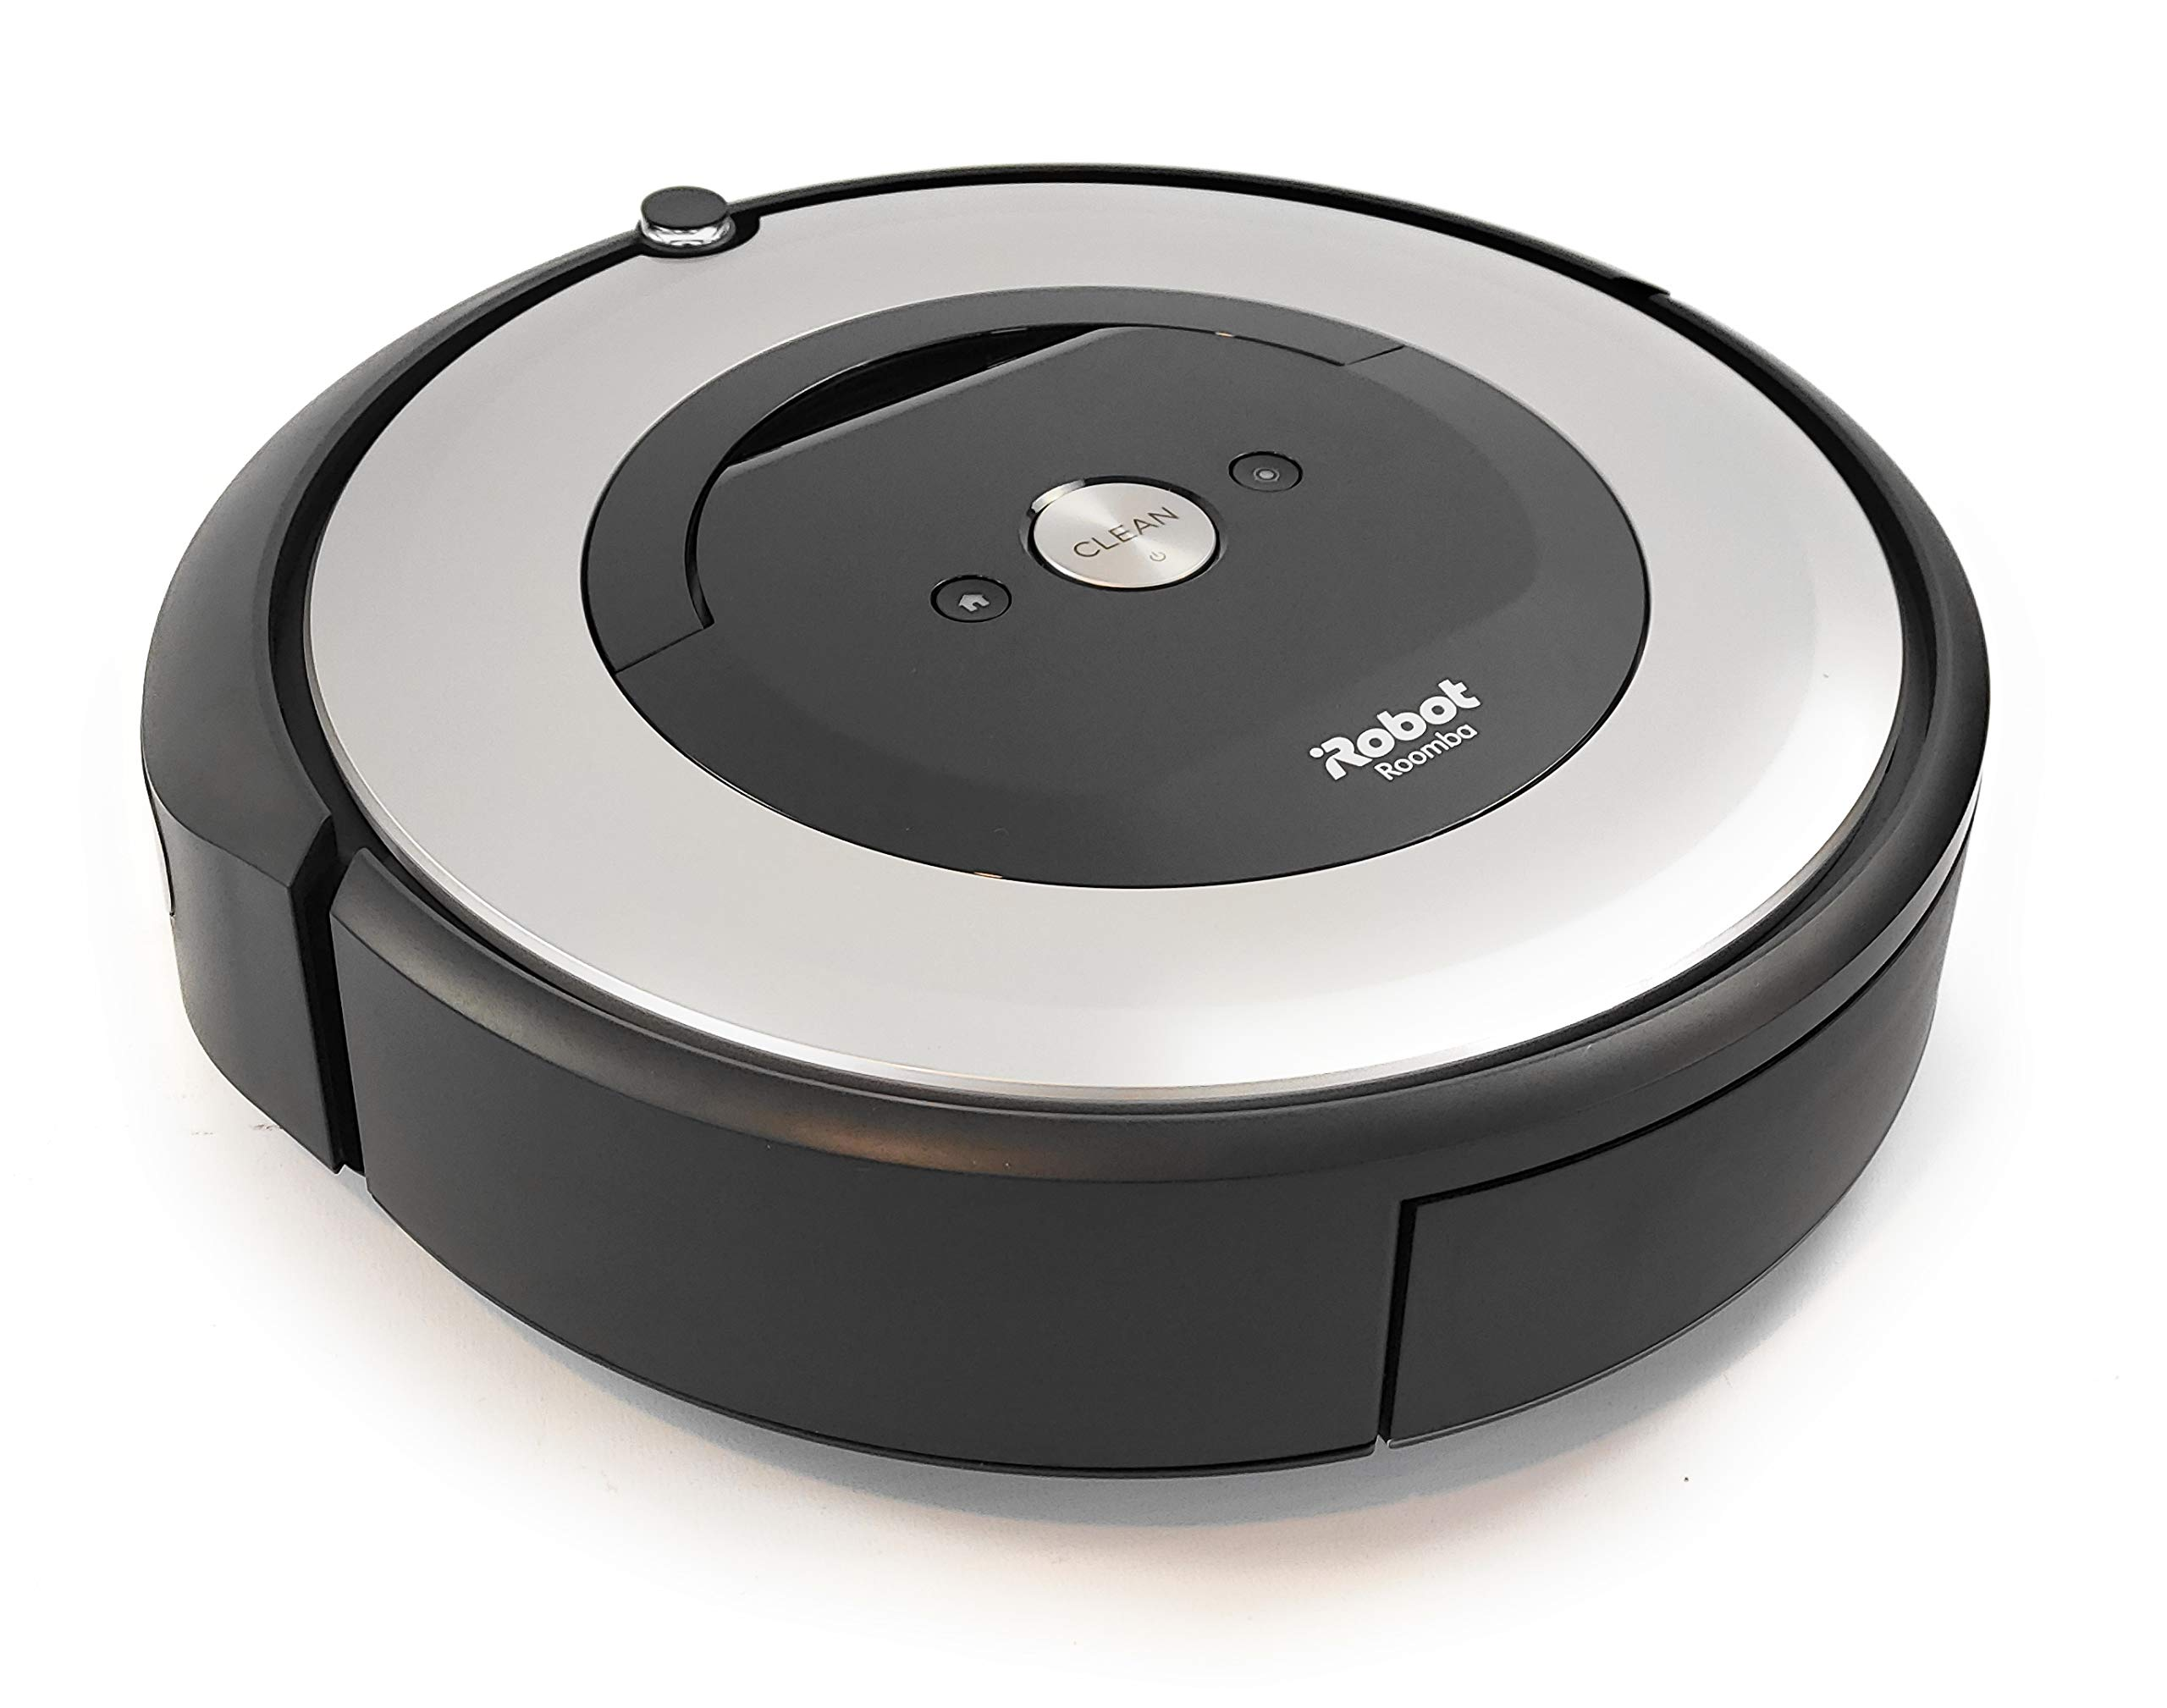
\includegraphics[width=0.5\textwidth]{figures/cap_1/roomba.jpg}
    \caption{Aspiradora autónoma}
    \label{fig:roomba}
\end{figure}

\begin{figure}[H]
    \centering
    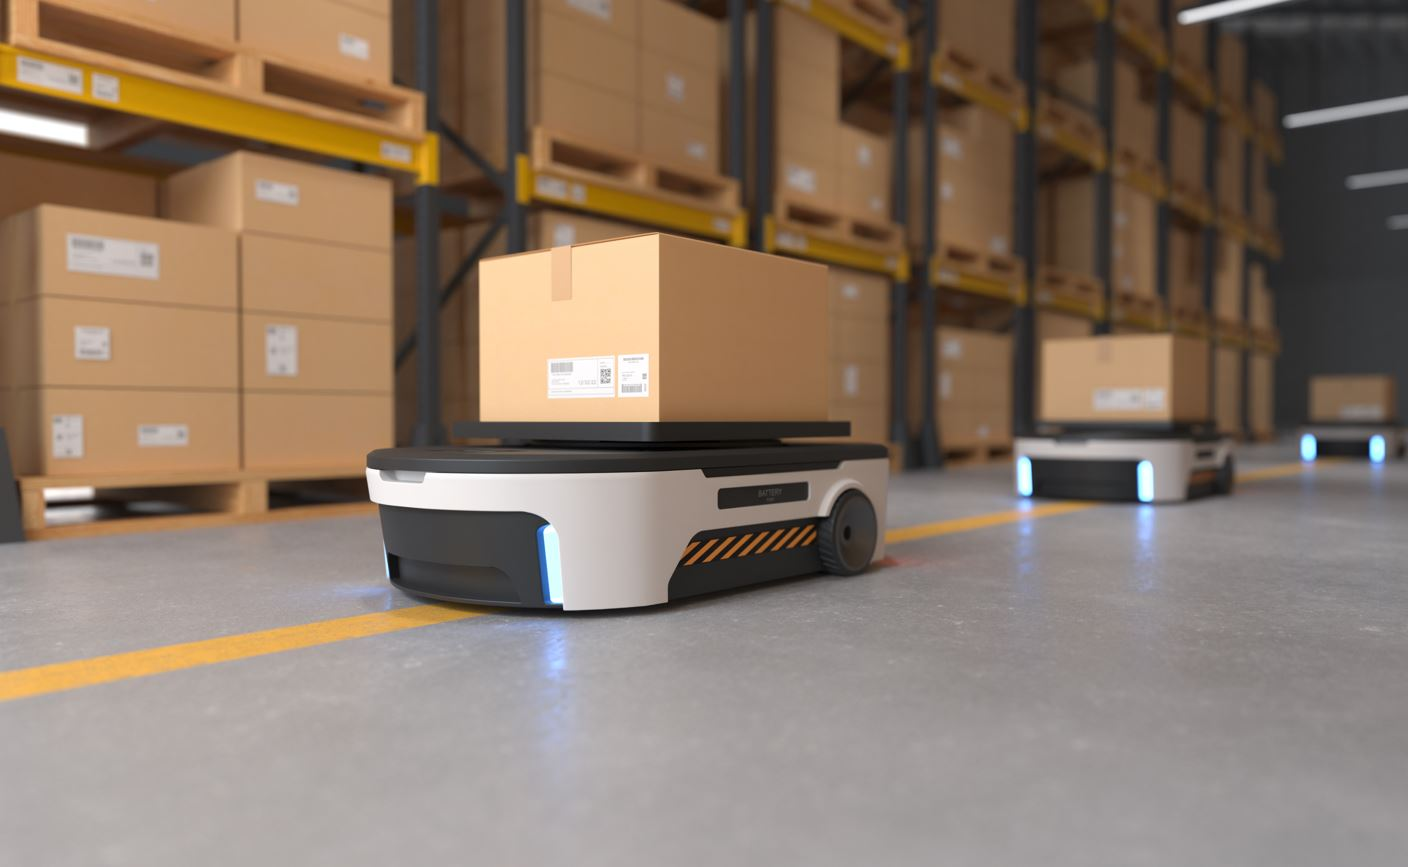
\includegraphics[width=0.7\textwidth]{figures/cap_1/agv.jpeg}
    \caption{Robot logístico AGV}
    \label{fig:agv}
\end{figure}

\begin{figure}[H]
    \centering
    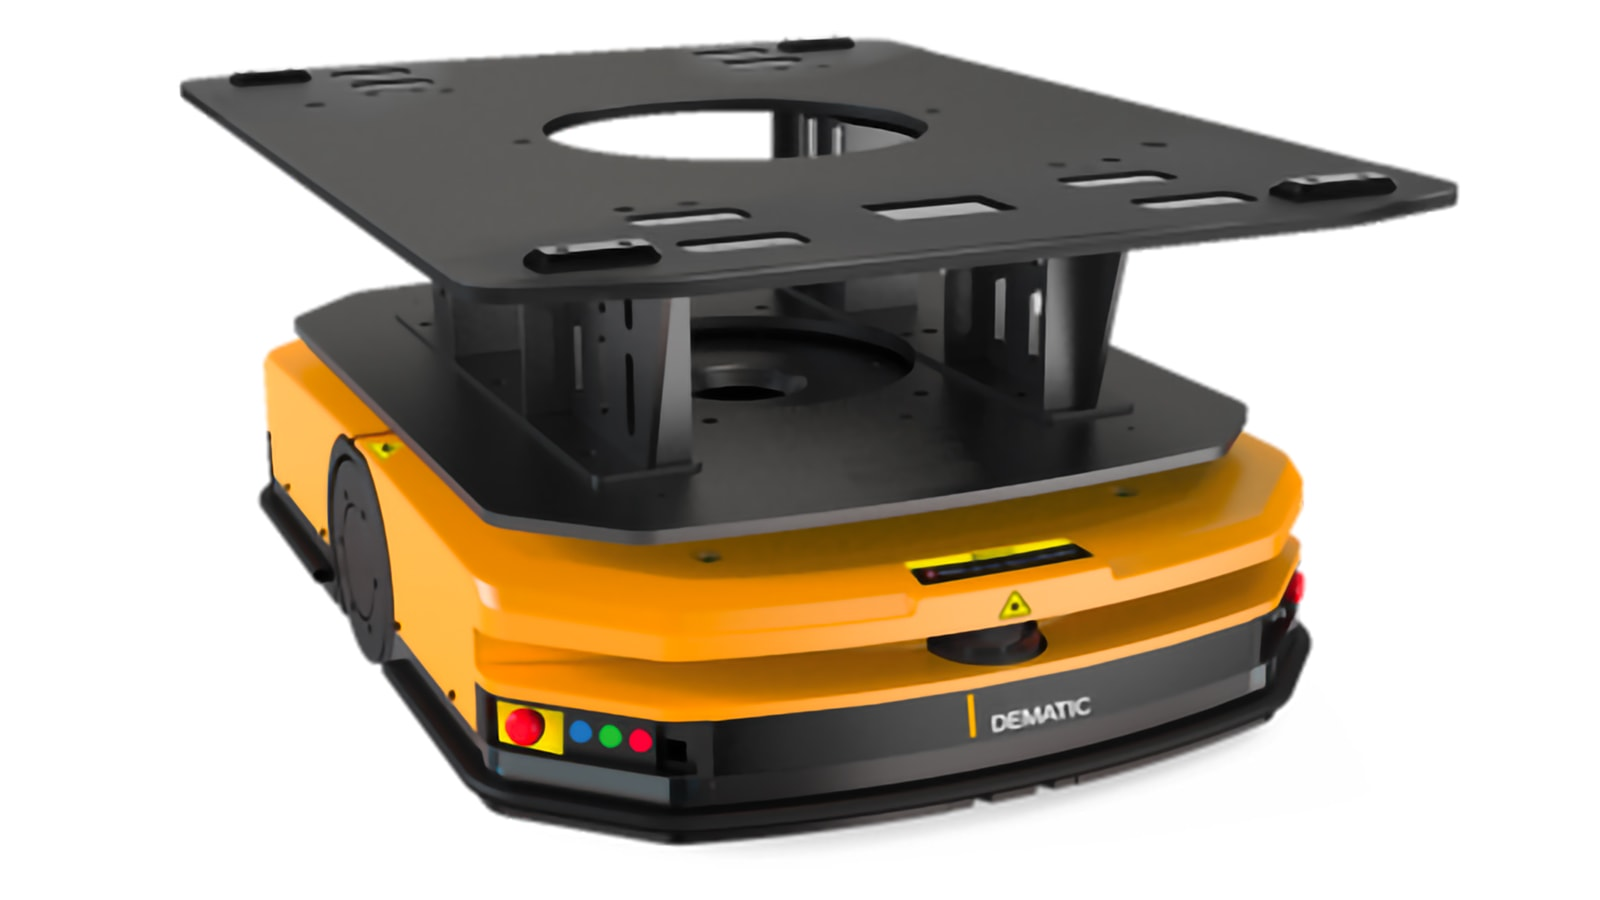
\includegraphics[width=0.7\textwidth]{figures/cap_1/amr.jpg}
    \caption{Robot logístico AMR}
    \label{fig:amr}
\end{figure}

\begin{figure}[H]
    \centering
    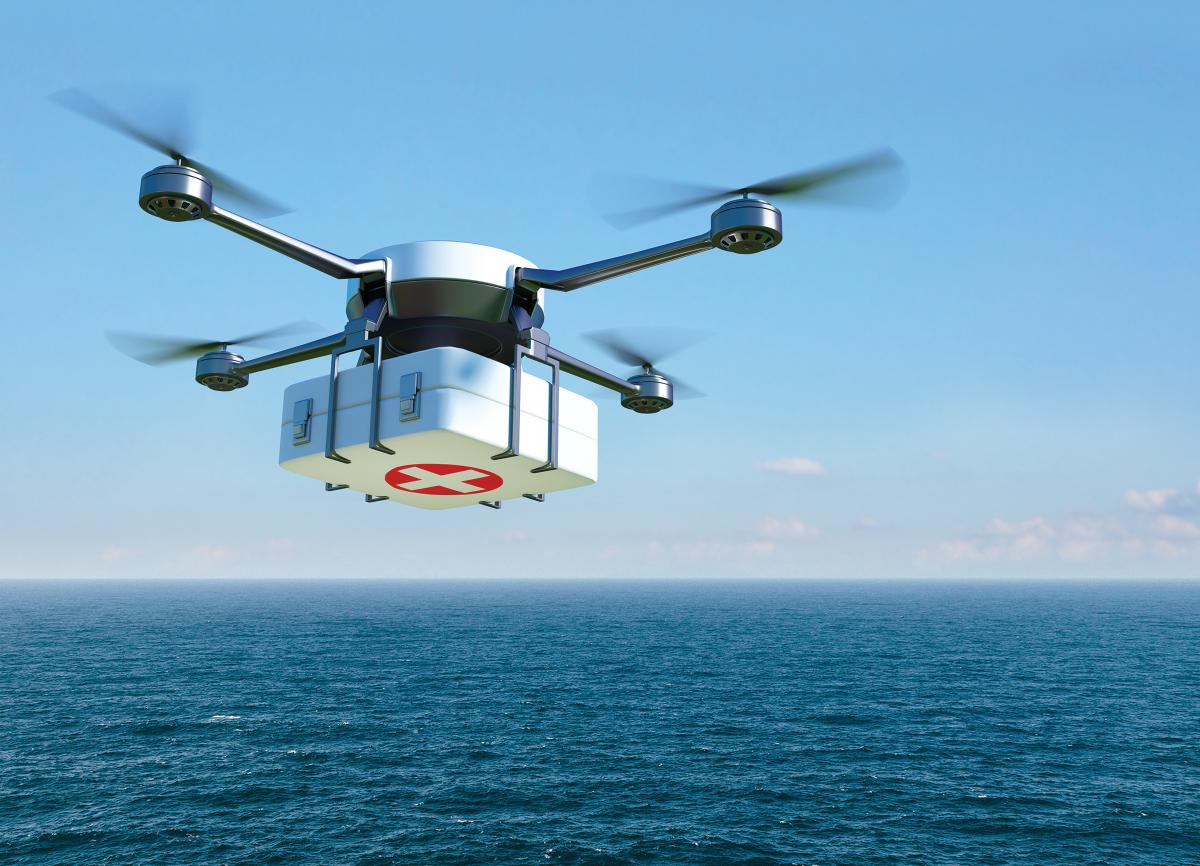
\includegraphics[width=0.7\textwidth]{figures/cap_1/dron.jpg}
    \caption{Dron de rescate}
    \label{fig:dron}
\end{figure}

\begin{figure}[H]
    \centering
    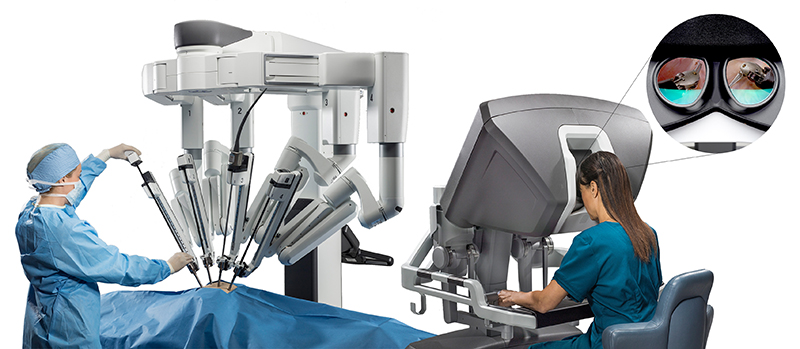
\includegraphics[width=0.9\textwidth]{figures/cap_1/davinci.jpg}
    \caption{Robot Da Vinci}
    \label{fig:davinci}
\end{figure}

Estos robots también se conocen como robots de consumo, y pueden clasificarse en dos categorías: personales y profesionales. Los primeros operan en el entorno doméstico, mientras que los segundos están diseñados para entornos empresariales, como fábricas, almacenes o zonas de construcción.

Es importante no confundirlos con los robots industriales, que suelen ser brazos robóticos fijos dedicados a realizar tareas repetitivas en un entorno controlado, como una línea de producción. Una excepción son los cobots (robots colaborativos), que están diseñados para interactuar directamente con personas en el ámbito industrial. Un ejemplo de estos robots son los de la empresa \textit{Universal Robots}\footnote{\url{https://www.universal-robots.com/es/}}, cuyos robots se muestran en la \autoref{fig:ur}.

\begin{figure}[H]
    \centering
    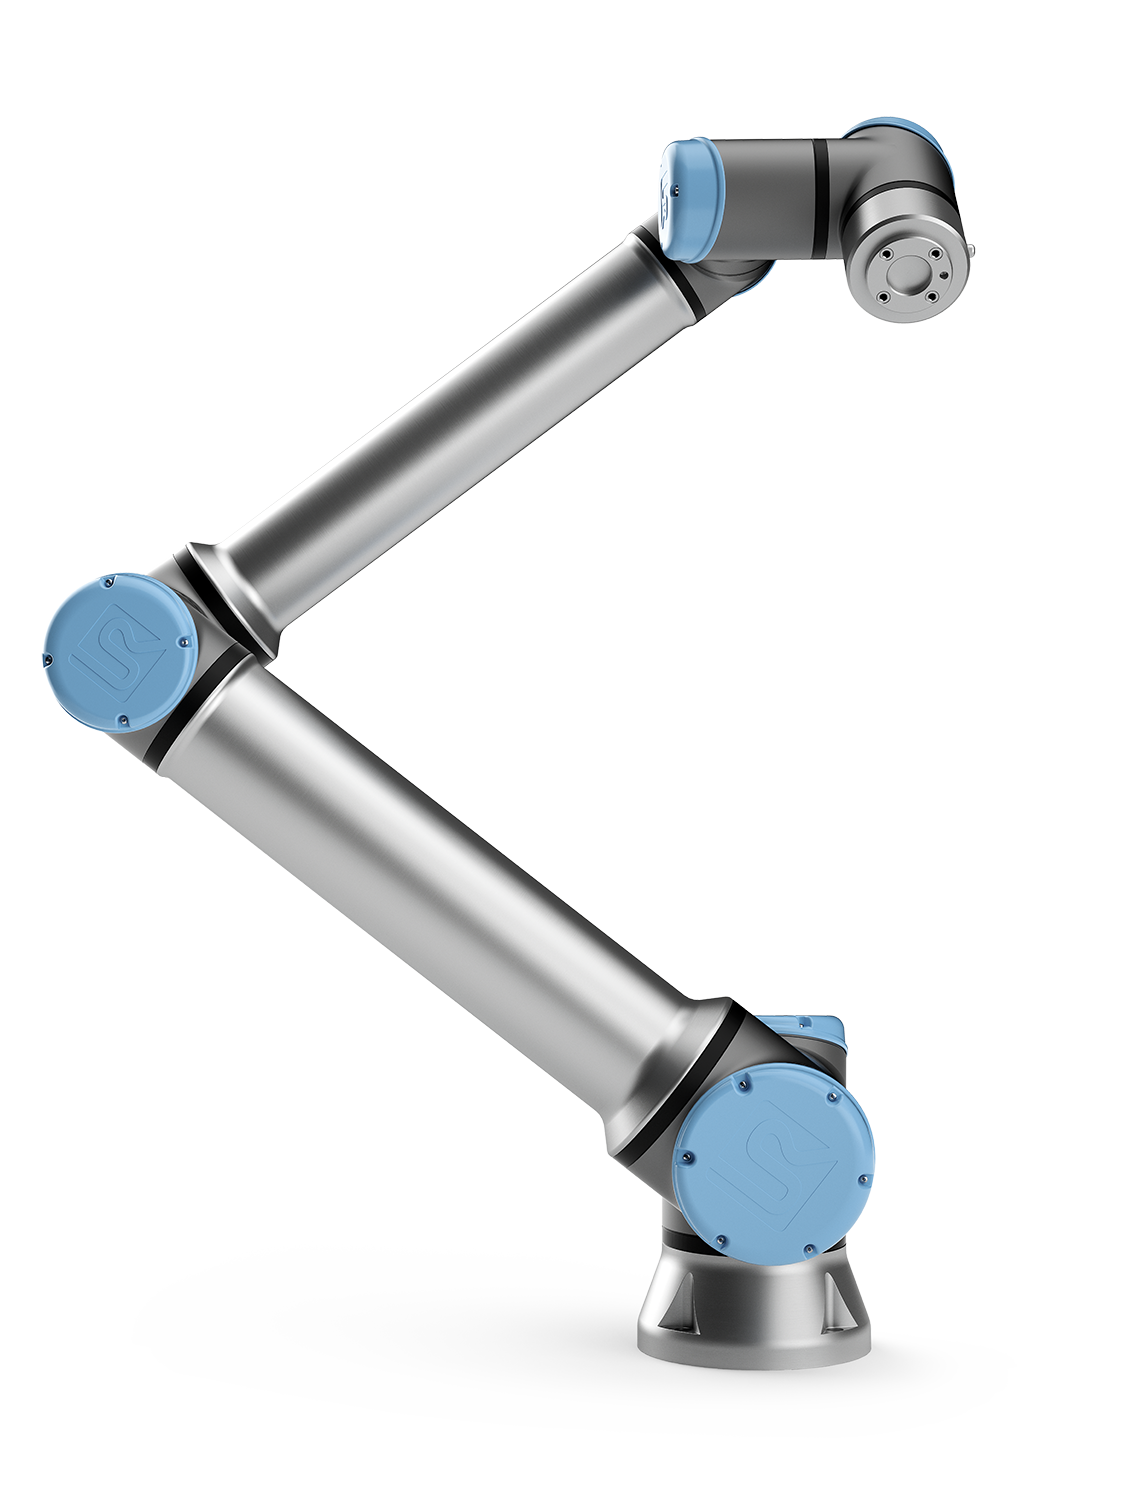
\includegraphics[height=0.7\textwidth]{figures/cap_1/ur10e.png}
    \caption{UR10e, Robot Colaborativo de Universal Robots}
    \label{fig:ur}
\end{figure}

A diferencia de los robots industriales, los robots de servicio o consumo deben desenvolverse en entornos no controlados, e incluso potencialmente hostiles. Además, no están necesariamente limitados a una sola tarea, ya que pueden adaptarse para realizar múltiples funciones y operar en distintos contextos.

\section{Robots Humanoides}

Dentro de los robots de servicio, destacan los robots humanoides, aquellos con la forma de su cuerpo construido para parecerse al cuerpo humano. Estos robots son especialmente interesantes a la hora de realizar tareas que ayuden a las personas. Esto es gracias a su diseño, que los hace lo suficientemente versátiles a la hora de realizar dichas tareas, ya que comparten la misma complexión y anatomía que los humanos.

Un ejemplo de este tipo de robots es el famoso Atlas\footnote{\url{https://bostondynamics.com/atlas/}}, de Boston Dynamics\footnote{\url{https://bostondynamics.com/}}. Este robot es completamente eléctrico y ha demostrado ser un robot extremadamente ágil, aunque no tanto como su predecesor, el robot Atlas hidráulico, capaz de moverse por entornos extremadamente complicados e incluso hacer acrobacias complejas. Ambos robots pueden verse en la \autoref{fig:atlas_electrico} y en la \autoref{fig:atlas_hidraulico}, respectivamente. También se adjuntan vídeos\footnote{\url{https://www.youtube.com/watch?v=I44_zbEwz_w}}\footnote{\url{https://www.youtube.com/watch?v=tF4DML7FIWk}} de lo que estos robots son capaces de hacer, también respectivamente.

\begin{figure}[H]
    \centering
    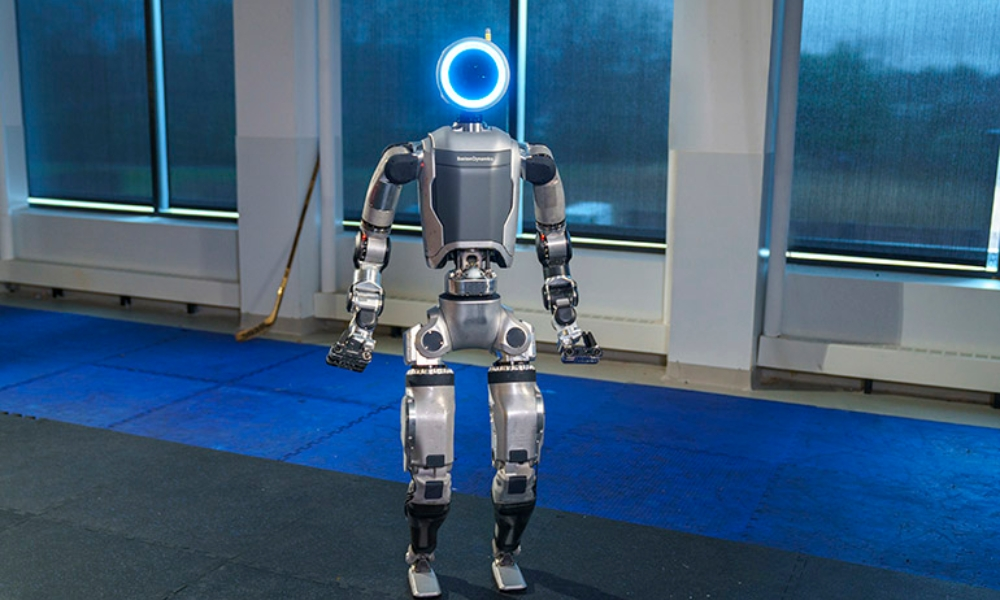
\includegraphics[width=0.8\textwidth]{figures/cap_1/atlas_electrico.jpg}
    \caption{Robot Atlas Eléctrico}
    \label{fig:atlas_electrico}
\end{figure}

\begin{figure}[H]
    \centering
    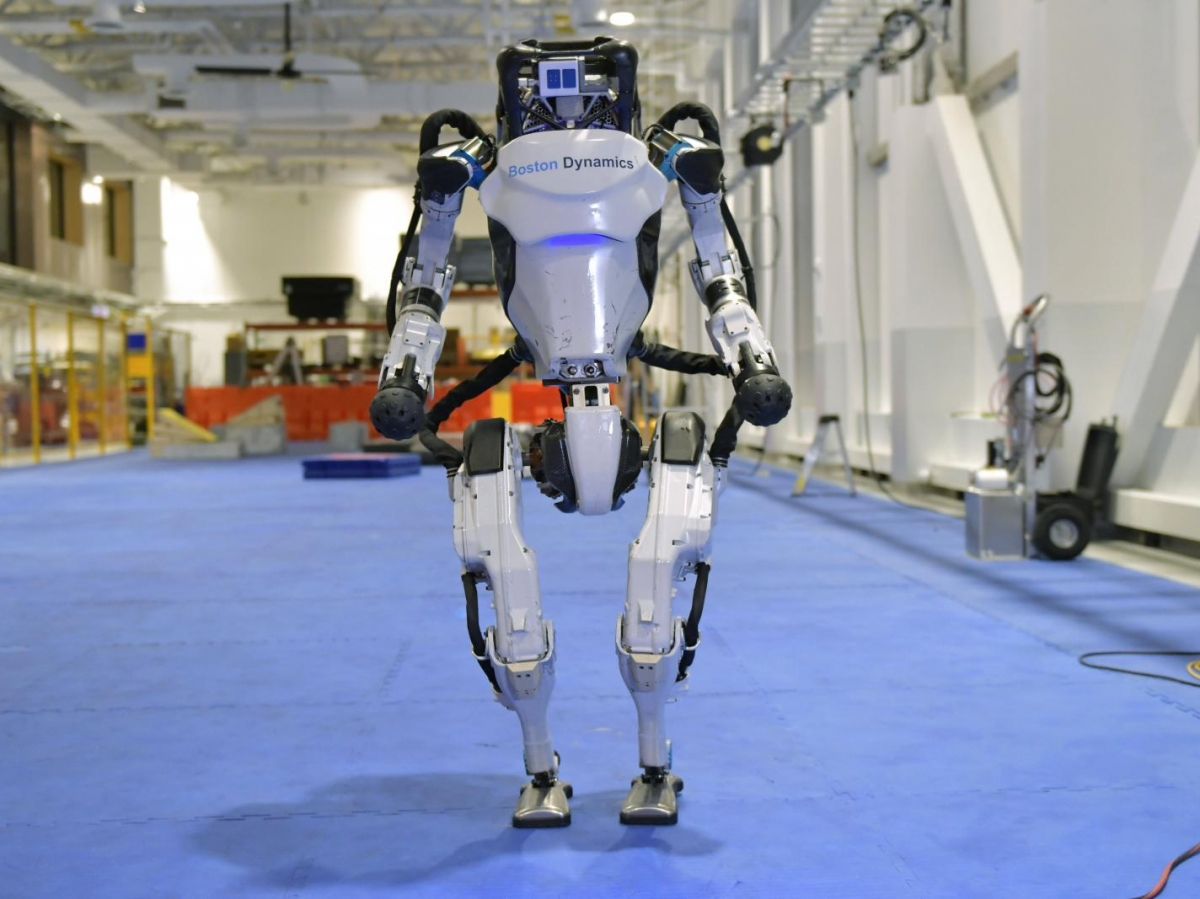
\includegraphics[width=0.8\textwidth]{figures/cap_1/atlas_hidraulico.jpg}
    \caption{Robot Atlas Hidráulico}
    \label{fig:atlas_hidraulico}
\end{figure}

Pero Atlas no es el único robot humanoide que existe, también tenemos al robot de Tesla\footnote{\url{https://www.tesla.com/es_es}}, Optimus\footnote{\url{https://www.tesla.com/es_es/we-robot}}, que también ha demostrado ser un robot bastante potente capaz de hacer varias tareas. Se muestra a continuación este robot en la \autoref{fig:optimus} y un vídeo\footnote{\url{https://www.youtube.com/watch?v=cpraXaw7dyc}} para conocerlo mejor.  

\begin{figure}[H]
    \centering
    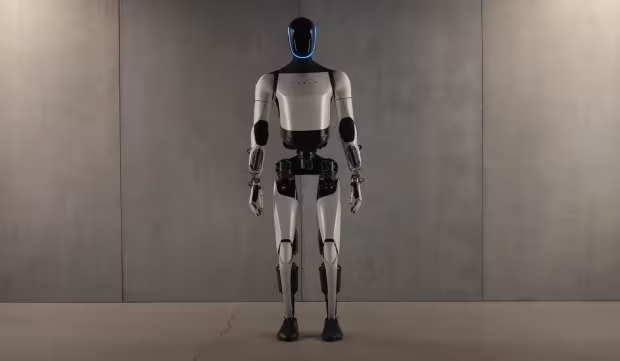
\includegraphics[width=0.8\textwidth]{figures/cap_1/optimus.jpg}
    \caption{Robot Optimus}
    \label{fig:optimus}
\end{figure}

Estos robots son demostradores, que sirven para enseñar hasta dónde somos capaces de llegar con la tecnología más puntera (pero no quiere decir que en el futuro se conviertan en robots de servicio masivos, cosa que aún nos queda un poco lejos).

Robots de servicio humanoides hay pocos, sin embargo, sí existen. Como ejemplo de este hecho tenemos a Digit\footnote{\url{https://www.agilityrobotics.com/solution}}, de Agility Robotics\footnote{\url{https://www.agilityrobotics.com/}}, un robot humanoide destinado a la logística que ha demostrado cumplir bastante bien con su tarea; para demostrarlo, se deja a continuación un vídeo\footnote{\url{https://www.youtube.com/watch?v=q8IdbodRG14}} donde lo vemos actuar. También se adjunta una fotografía de este robot en la \autoref{fig:digit}.

\begin{figure}[H]
    \centering
    \includegraphics[width=0.8\textwidth]{figures/cap_1/digit.jpg}
    \caption{Robot Digit}
    \label{fig:digit}
\end{figure}

Sin embargo, aunque estos robots son construibles en la vida real, suponen una dificultad muy alta, ya que hay que tener en cuenta muchos factores y desafíos.

Estos desafíos residen especialmente en la locomoción, ya que, al moverse mediante piernas, deben ser estables tanto estática cómo dinámicamente. También deben tener una anatomía adecuada y un aspecto amigable para los humanos, lo que conlleva esquivar \textit{el valle inquietante}, un punto en el que los robots son tan realistas que causan rechazo, e incluso miedo en algunos casos. Es por eso que los que hemos visto anteriormente no son tan antropomórficos ni realistas. 

También como desafío están el tamaño y el peso del robot, que, al ser de un tamaño grande, hay que compensar los pesos adecuadamente para conseguir esa estabilidad estática que se mencionaba anteriormente. En cuanto a la estabilidad dinámica, esto requiere mucho tiempo de entrenamiento del robot en cuanto a modos de caminar, cosa que se suele hacer mediante entrenamiento por refuerzo en simuladores.

Cómo último ejemplo de robot humanoide se hace referencia al robot NAO\cite{pagina_nao}, de Aldebaran, ahora Softbank Robotics\footnote{\url{https://us.softbankrobotics.com/}}. Protagonista de este TFG.

Este robot es el pequeño humanoide de 4,3 kg de peso y 58 cm de altura que se puede ver en la \autoref{fig:nao}.

\begin{figure}[H]
    \centering
    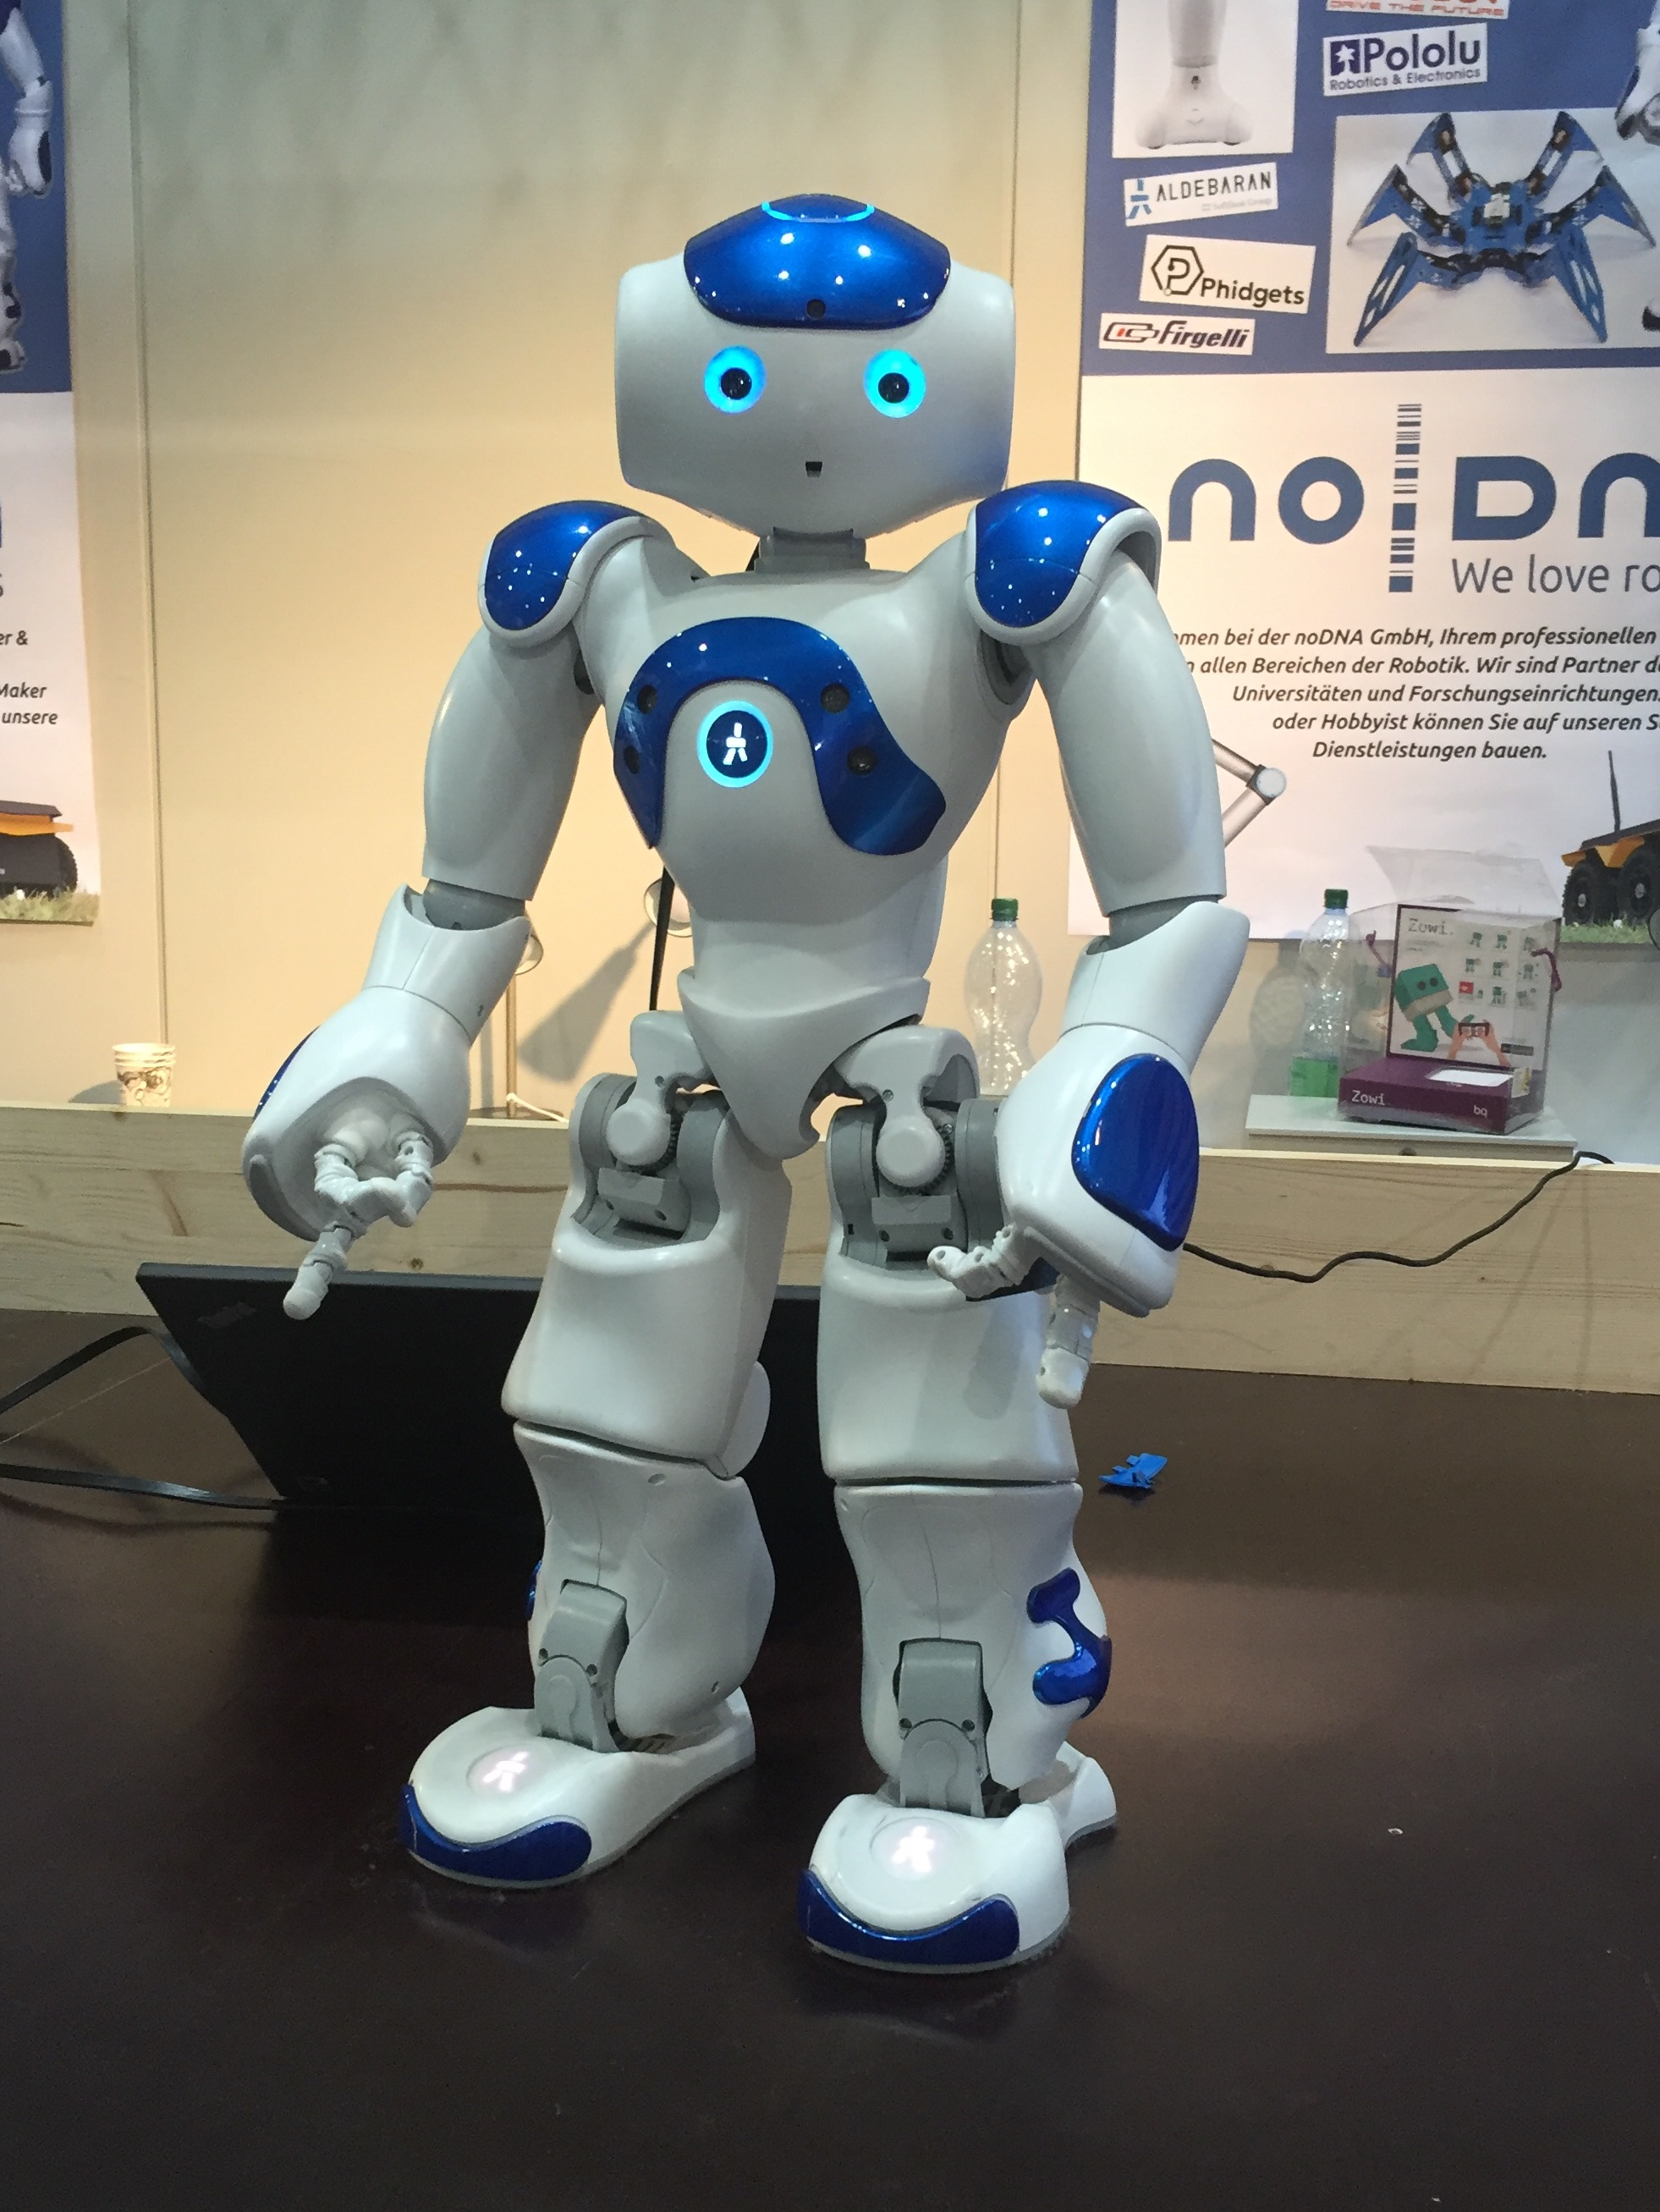
\includegraphics[width=0.5\textwidth]{figures/cap_1/nao.jpg}
    \caption{Robot NAO}
    \label{fig:nao}
\end{figure}

Sin embargo, este robot no es un robot de servicios. Es un robot principalmente educativo, destinado a que las personas aprendan las bases de la robótica y la programación mientras lo usan, además de ser divertido para los niños e interesante para la investigación. De hecho, este robot fue la liga de hardware estandard dentro de la RoboCup soccer\footnote{\url{https://www.robocup.org/leagues/5}} durante 17 años consecutivos, desde 2008 hasta 2024.

Este robot también ha protagonizado muchos trabajos de fin de grado anteriores, por ser el humanoide más accesible tanto por nuestra universidad (por tenerlo en el laboratorio), como por los estudiantes individualmente al poder acceder a su modelo simulado. Ejemplos de dichos trabajos pueden apreciarse en \cite{tfg_caminata_nao} y  \cite{tfg_caminatas_ondas}, dónde se utiliza este robot para explorar  modos de caminar, un problema muy común en humanoides y muy interesante para investigar debido a su elevada complejidad.

Cabe destacar también que este robot es muy versátil a la hora de programarlo, ya que se puede optar por su forma predeterminada mediante Naoqui\footnote{\url{http://doc.aldebaran.com/1-14/dev/naoqi/index.html}}, un \textit{framework} específico para programar al robot mediante programación visual que puede verse en la \autoref{fig:naoqui}. Pero también ofrece la posibilidad de programarlo mediante el uso de ROS2, como se hará en este TFG o bien utilizando otros medios como por ejemplo el simulador Webots, al que haremos refrencia en el capítulo \ref{cap:herramientas}.

\begin{figure}[H]
    \centering
    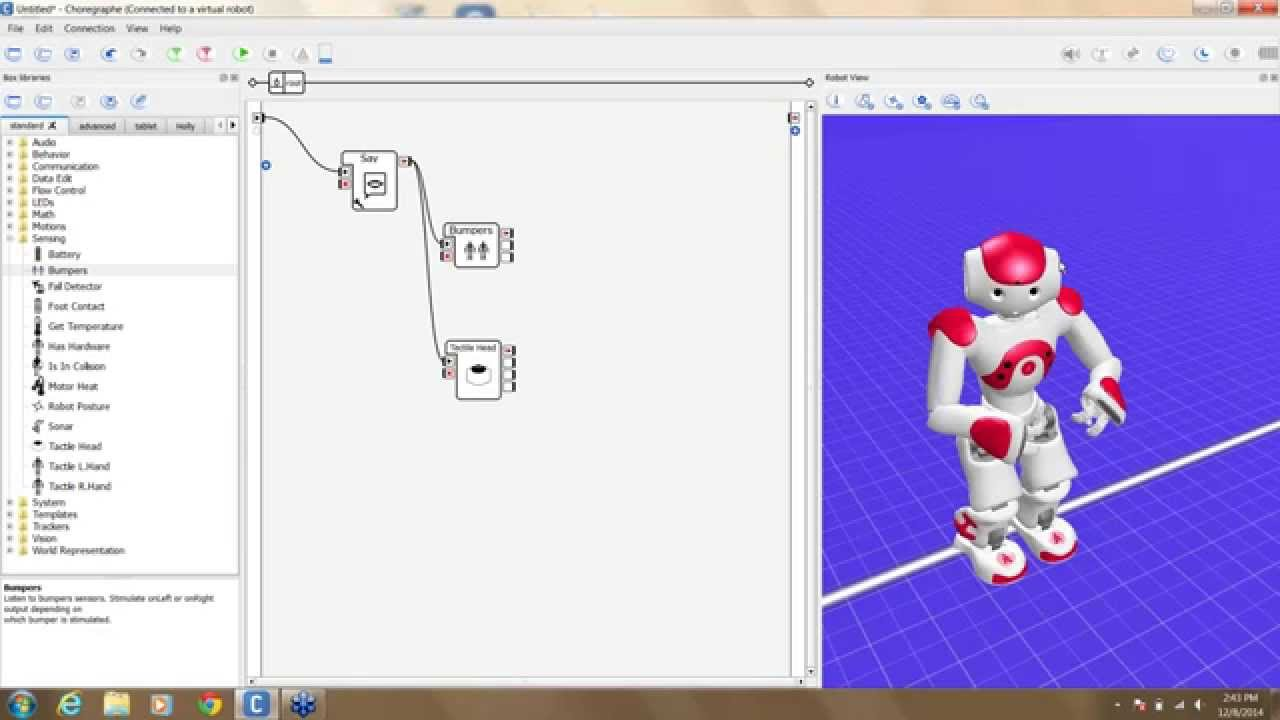
\includegraphics[width=1\textwidth]{figures/cap_1/naoqui.jpg}
    \caption{Lenguaje Naoqui}
    \label{fig:naoqui}
\end{figure}

\section{Simuladores Robóticos}

Los simuladores son aplicaciones software que permiten emular \textit{via software} de manera realista al robot y su entorno, lo que los convierte en una herramienta extremadamente útil a la hora de construir todo tipo de robots, ya que evitan posibles catástrofes en la realidad a la hora de usarlos, por ejemplo, si un robot cae en el entorno simulado, sus componentes reales quedarán a salvo. Es por eso por lo que tienen mucha importancia a la hora del desarrollo de robots humanoides, debido a su elevado coste y complicación a la hora de construirlos. Los simuladores también son útiles para entrenar dichos robots en diferentes ámbitos y escenarios, para así brindarles la máxima versatilidad posible y que puedan realizar casi cualquier tarea que podría hacer un humano.

Existen muchos simuladores robóticos, entre los que destacan el simulador de NVIDIA\footnote{\url{https://www.nvidia.com/es-es/}}, Isaac Sim\footnote{\url{https://developer.nvidia.com/isaac/sim}}, capaz de entrenar un robot para que aprenda a caminar en sólamente 2 horas, según lo indicado por CyberRobo en la plataforma X\footnote{\url{https://x.com/CyberRobooo/status/1921252216330912032}}. 

Otro simulador muy presente en la actualidad es Coppelia Sim\footnote{\url{https://www.coppeliarobotics.com/}}, un simulador utilizado en la industria, la educación y la investigación. Originalmente fue desarrollado dentro del departamento de I+D de Toshiba\footnote{\url{https://www.toshiba.es/}} y actualmente está siendo desarrollado y mantenido activamente por Coppelia Robotics AG\footnote{\url{https://github.com/CoppeliaRobotics}}, una pequeña empresa ubicada en Zúrich, Suiza. Este simulador ha resultado muy útil para simulación de robots móviles con navegación autónoma, Robots que usan SLAM para mapear un entorno, brazos robóticos con \textit{pick and place}, e incluso simulación de robots humanoides caminantes.

También existe el simulador Webots, un simulador \textit{opensource} educativo en el que se hará más incapié en el capítulo \ref{cap:herramientas}.

Por último, destaca también Gazebo, simulador específico para ROS2, muy potente y además \textit{opensource}. Éste es el simulador que se utilizará para el desarrollo de este TFG. Se hablará más en profundidad sobre él en el Capítulo \ref{cap:herramientas}.

Todo lo expuesto en este capítulo ha sido clave para decidir como objetivo dotar al robot NAO simulado en Gazebo de una librería de coordinación de actuadores que le permita caminar (especialmente por el desafío técnico que supone) y, además, programar una aplicación en el contexto de un invernadero como validación experimental de la biblioteca de movimientos y de su potencial uso como robot de servicio.
    \chapter{Objetivos}\label{cap:objetivos}

\section{Problema a resolver}

Como se ha introducido en el Capítulo~\ref{cap:introduccion}, el objetivo principal de este TFG es dotar al humanoide NAO de una capa completa de movimientos y locomoción, para luego programar una aplicación que empleará este robot educativo en el ámbito de la robótica de servicios. Esta aplicación servirá además de validación para demostrar que dicha capa de movimiento es funcional e intuitiva de utilizar.

Sin embargo, este objetivo es muy general y amplio, así que lo mejor es dividirlo en subobjetivos, que se detallan a continuación.

\begin{itemize}
    \item \textit{Subobjetivo 1}: Como primer subobjetivo tenemos el ser capaces de crear patrones fijos de movimiento y que NAO pueda replicarlos fielmente y con los menores errores posibles.
    \item \textit{Subobjetivo 2}: El segundo subobjetivo de este proyecto es dotar al humanoide de la capacidad de parametrizar sus movimientos y  poder ofrecer modos de caminar distintos y con la velocidad variable, obteniendo así movimientos continuos parametrizables. Estos movimientos deben encapsularse en una librería para que su uso sea más sencillo y directo. Dicha librería contendrá además toda la funcionalidad de ROS2 y los patrones fijos ofrecidos por el robot, para que así sea una biblioteca utilizable por cualquier usuario de manera sencilla.
    \item \textit{Subobjetivo 3}: Como tercer y último subobjetivo, tenemos el desarrollar una aplicación que sirva de demostradora de la potencia de dicha libería, haciendo que el robot preste servicio en un invernadero.

    El servicio que debe ofrecer es similar al visto en el robot Digit, esto es, mover una caja de un lugar de origen a uno de destino, pero, en lugar de en un almacén, se hará en un invernadero para dar más identidad y originalidad al proyecto.
\end{itemize}

\section{Metodología}

Para alcanzar los subobjetivos planteados y, en última instancia, cumplir con el objetivo principal del proyecto, se ha optado por adoptar la metodología \textit{Scrum} como marco de trabajo. Esta elección responde a la necesidad de mantener una dinámica de desarrollo iterativa y adaptable (Esquema del funcionamiento de esta metodología en la \autoref{fig:scrum}). 

\begin{figure}[H]
    \centering
    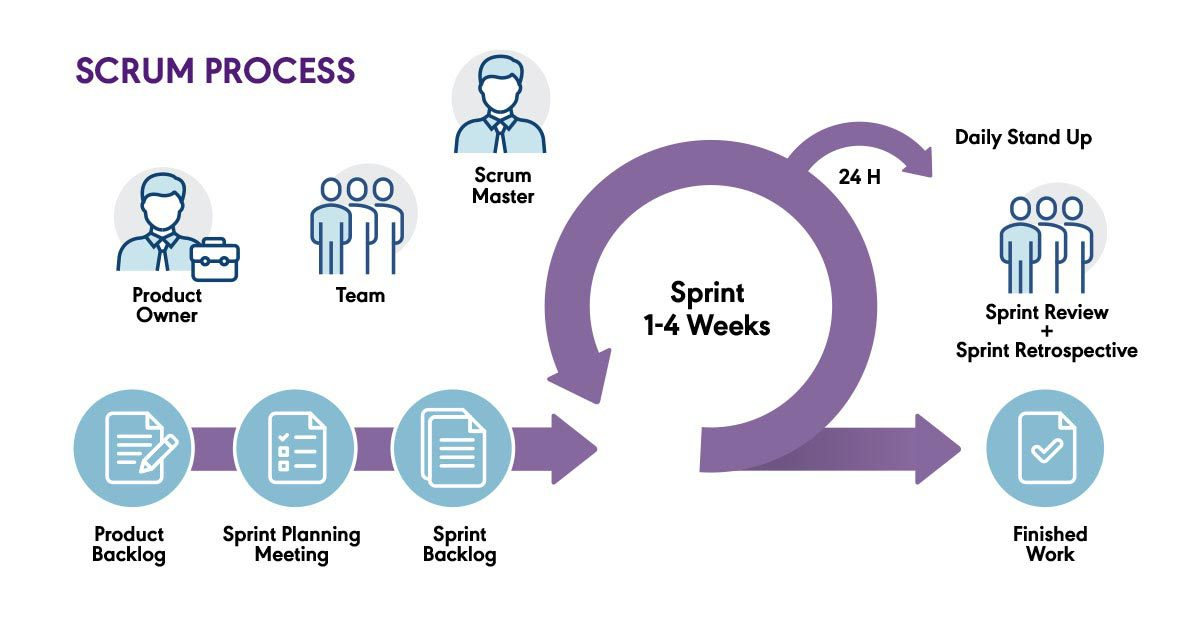
\includegraphics[width=1\textwidth]{figures/cap_2/scrum.jpg}
    \caption{Esquema del funcionamiento de la metodología \textit{Scrum}}
    \label{fig:scrum}
\end{figure}

En este contexto, se han establecido reuniones semanales con el tutor del proyecto, que cumplen la función de revisiones periódicas del progreso similares a las \textit{Sprint Reviews}, ya que, durante estas sesiones, se evalúan los avances logrados en la última iteración y se definen de manera colaborativa los siguientes pasos a seguir. Este enfoque permite ajustar la planificación de forma continua en función de los resultados obtenidos, fomentar la mejora progresiva del proyecto, y asegurar que cada etapa del desarrollo esté alineada con los objetivos generales. De esta manera, se garantiza un proceso flexible, enfocado en la entrega constante de valor y la toma de decisiones informadas a lo largo del ciclo de desarrollo.

En resumen, la metodología que se ha aplicado estaba basada en \textit{sprints} de \textit{Scrum} semanales los cuales iba marcando mi tutor, en función a los objetivos cumplidos del sprint anterior.

\subsection{Plan de trabajo}

El primer \textit{sprint} de trabajo fue elegir una plataforma para alojar el proyecto y facilitar el seguimiento del mismo.

Para cumplir con eso, se ha decidido alojar el código fuente generado en un repositorio de GitHub\footnote{\url{https://github.com/}}, plataforma que ayuda a los desarrolladores a almacenar y gestionar su código, así como a rastrear y controlar los cambios en él, lo que lo convierte en la plataforma de control de versiones preferida a la hora de desarrollar proyectos grandes, como es el caso de este TFG.

Que sea un sistema de control de versiones nos ayuda a tener registradas todas y cada una de las versiones del proyecto, pudiendo volver a una versión anterior o seguir avanzando a placer. Esto es de gran ayuda por si es necesario volver a una versión anterior por cualquier razón.

El repositorio dónde se aloja este proyecto\footnote{\url{https://github.com/RoboticsLabURJC/2024-tfg-eva-fernandez}} sigue la siguiente estructura:

\begin{itemize}
    \item \textit{Directorio CoordMoves}: Es en este directorio donde se aloja el proyecto completo, códigos, modelos, mundos, este documento, etc.
    \item \textit{Directorio pruebas}: En este directorio fue donde se trabajó durante la fase experimental del proyecto, con todo lo que eso conlleva. 
    \item \textit{Directorio docs}: Directorio dónde se aloja un blog de seguimiento semanal del proyecto, lo trataremos con profundidad más adelante.
    \item Fichero \textit{README.md}: Un fichero en el que se describe de forma resumida todo el proyecto, ya que éste es público.
\end{itemize}

También se ha decidido utilizar Github Pages\footnote{\url{https://pages.github.com/}}, un servicio de alojamiento de sitios estáticos que toma archivos HTML, CSS y JavaScript directamente de un repositorio en GitHub, los ejecuta opcionalmente mediante un proceso de compilación y publica un sitio web. Ha sido utilizado en el proyecto para llevar un blog semanal\footnote{\url{https://roboticslaburjc.github.io/2024-tfg-eva-fernandez/}}, en el que se comentan avances, percances o ideas que han surgido durante el desarrollo del proyecto, desde su inicio, hasta su fin.

Este blog es una forma muy potente de documentar el proceso de desarrollo y poder seguir el esquema \textit{Scrum}, ya que, no sólo es interesante para ver cómo se ha hecho o qué se ha hecho, si no que ha servido de mucha ayuda para que mi tutor tuviera un seguimiento más rígido del proceso y se pudieran abarcar todas las cuestiones y avances realizados en las reuniones.

Los sprints siguientes fueron más variados, cómo buscar un modelo, prepararlo junto a un primer mundo, descubrir cómo controlar este modelo con ROS2, etc. Lo que nos dejó 3 fases principales a la hora del desarrollo:

\begin{itemize}
    \item \textit{Fase 1}: Preparación del modelo y un mundo vacío
    \item \textit{Fase 2}: Desarrollo de un intérprete de movimientos y un editor
    \item \textit{Fase 3}: Implementación de la librería y llenado del mundo
    \item \textit{Fase 4}: Desarrollo de la aplicación
\end{itemize}
    \chapter{Herramientas Software utilizadas}\label{cap:herramientas}

 En este capítulo, se explicarán las herramientas software utilizadas para llevar a cabo este TFG, es decir, se comentarán los recursos que han servido para la programación y estructuración del proyecto.

\section{Ecosistema: Middleware ROS 2}

ROS\footnote{\url{https://www.ros.org/}} es un middleware que ofrece un conjunto de bibliotecas y herramientas de software que ayudan a crear aplicaciones robóticas. Desde controladores hasta algoritmos de vanguardia, y con potentes herramientas de desarrollo, tiene todo lo necesario para consruir un proyecto de robótica. Y todo es de código abierto.

Tiene dos versiones, ROS (también conocida cómo ROS1, es la primera que salió y la más antigua) y ROS2, la más moderna y la que ha sido utilizada para este proyecto. Además de ser el middleware por excelencia utilizado a lo largo de la carrera por diferentes asignaturas, ROS2 es una potente herramienta utilizada alrededor del mundo para manejar robots.

Dispone de varias distribuciones que van saliendo cada cierto tiempo, cada una compatible con una distribución de Ubuntu concreta. En mi caso, se ha utilizado la anterior dsitribución de ROS2, Humble Hawksbill\footnote{\url{https://docs.ros.org/en/humble/Installation.html}}, debido a que la distribución Ubuntu utilizada ha sido la 22.04 LTS, distribución directamente compatible con Humble.

Para trabajar con ROS, es necesario crear paquetes \cite{tutorial_paquete} para alojar los diferentes programas para publicar o suscribirse a los \textit{topics} del robot \cite{tutorial_pubsub} y especificaciones necesarias para la aplicación robótica a desarrollar, y pueden crearse directamente para los lenguajes C++, o Python, de los cuales se ha optado por el segundo.

\section{Lenguaje de programación: Python}

Como bien se ha dicho anteriormente, el lenguaje de programación utilizado ha sido Python\footnote{\url{https://www.python.org/}}, lenguaje de alto nivel de programación interpretado cuya filosofía hace hincapié en la legibilidad de su código. Se trata de un lenguaje de programación multiparadigma, ya que soporta parcialmente la orientación a objetos, programación imperativa y, en menor medida, programación funcional. Es un lenguaje interpretado, dinámico y multiplataforma.

Se ha optado por este lenguaje porque está ampliamente extendido y es fácil de interpretar y utilizar, además de que es compatible con ROS2, pudiendo crear paquetes directamente para este lenguaje. La versión utilizada ha sido la 3.10, versión por defecto instalada en Ubuntu 22.04.

\section{Simulador Gazebo}

Una vez elegidos el middleware y el lenguaje de programación, es necesario elegir un robot y un escenario. Cómo adquirir un robot es algo costoso y mi situación personal no permitía trabajar con los robots que ofrece nuestro laboratorio en la URJC, se optó por trabajar en un entorno completamente simulado.

Para ello, Gazebo\footnote{\url{https://gazebosim.org/home}} fue la mejor opción, por su directa compatibilidad con ROS2 y potencia de simulación, además de que, como ROS, es de código abierto.

A la hora de elegir la versión a utilizar, se decidió usar la versión más reciente del simulador, Gazebo Harmonic, para así no quedarnos tan atrás a la hora de desarrollar, ya que usábamos la versión anterior de ROS2.

\subsection{Modelo del robot NAO simulado}

Una vez escogido el entorno de simulación, era hora de buscar un robot adecuado para el proyecto. Como ya se ha mencionado, nuestro protagonista es el Robot NAO, de Aldebaran, por lo que era necesario encontrar un modelo en el formato de Gazebo (SDF) para poder hacerlo funcionar.

Para esto, Gazebo dispone de una amplia biblioteca\footnote{\url{https://app.gazebosim.org/dashboard}} de mundos y modelos ya creados por empresas o la comunidad, así que sólo era buscarlo en esta biblioteca.

Al final, el modelo utilizado sería el ofrecido por OpenRobotics, que se muestra a continuación:

\begin{figure}[H]
    \centering
    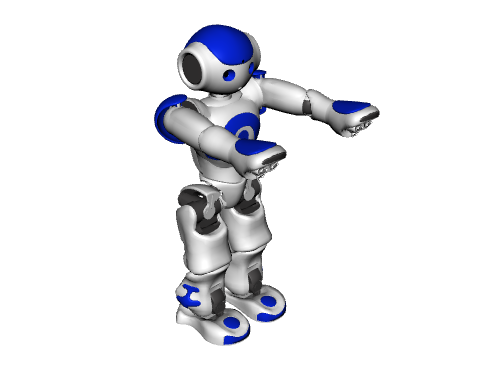
\includegraphics[width=0.5\textwidth]{figures/cap_3/modelo_original.png}
    \caption{Modelo del robot NAO utilizado}
    \label{fig:modelo_original}
\end{figure}

Este modelo\footnote{\url{https://app.gazebosim.org/OpenRobotics/fuel/models/NAO\%20with\%20Ignition\%20position\%20controller}} cuenta con un sistema de control de articulaciones ya construido, por lo que resulta perfecto para el proyecto. De hecho, el propio Gazebo Harmonic, al abrirse, tiene una demo que prueba este control de los \textit{joints} de este mismo modelo, cosa que puede verse en la \autoref{fig:inicio_gazebo}.

 A continuación se adjunta una captura de pantalla de dicha demostración (\autoref{fig:demo_gazebo}), así cómo un vídeo\footnote{\url{https://youtu.be/y6Rn2WOl_Xw}} para que se aprecie bien el funcionamiento.

\begin{figure}[H]
    \centering
    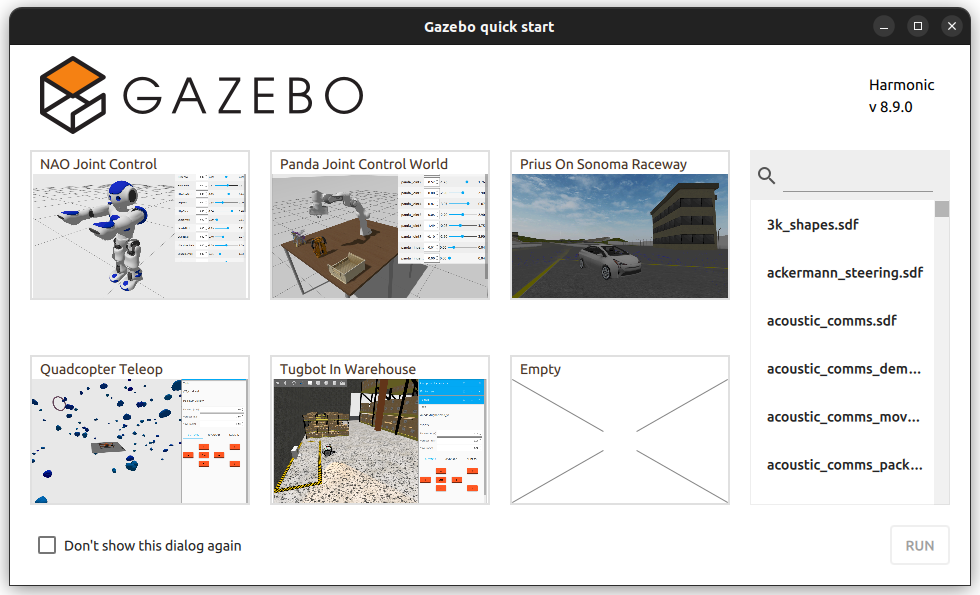
\includegraphics[width=1\textwidth]{figures/cap_3/inicio_gazebo.png}
    \caption{Inicio de Gazebo Harmonic, para acceder a la demo de control del NAO}
    \label{fig:inicio_gazebo}
\end{figure}

\begin{figure}[H]
    \centering
    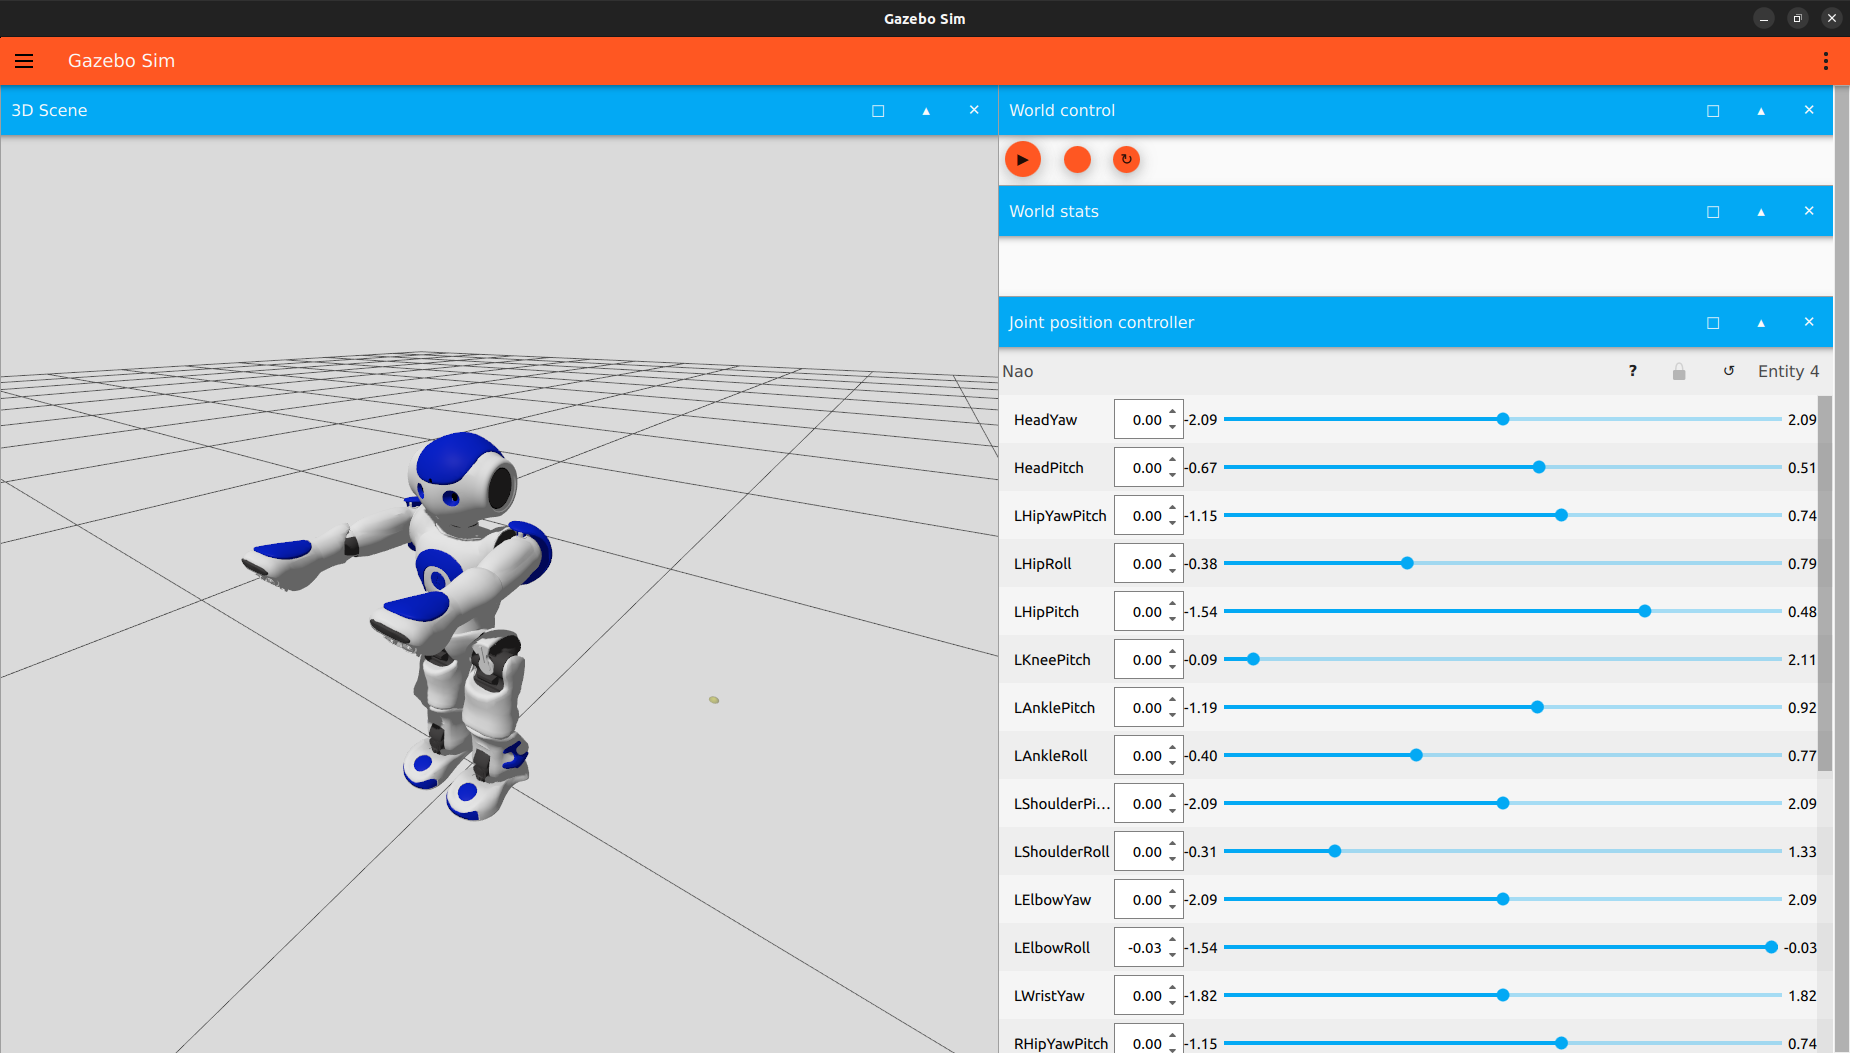
\includegraphics[width=1\textwidth]{figures/cap_3/demo_nao.png}
    \caption{Demo de Gazebo Harmonic para control de las articulaciones de NAO}
    \label{fig:demo_gazebo}
\end{figure}

El soporte básico de este modelo es ofrecer acceso a los actuadores de las articulaciones individualmente, sin embargo, no ofrece ningún mecanismo de coordinación o locomoción  que involucre a varias articulaciones de forma ordenada o coordinada. Pero el uso de Gazebo y este modelo en particular es necesario para probar los mecanismos de coordinación desarrollados en este TFG, y también para dotar al robot de un escenario para validar la aplicación robótica creada.

\section{Simulador Webots}

Webots\footnote{\url{https://cyberbotics.com/}} es una aplicación de escritorio multiplataforma de código abierto que se utiliza para simular robots. Proporciona un entorno de desarrollo completo para modelar, programar y simular robots.

Diseñado para uso profesional, se utiliza ampliamente en la industria, la educación y la investigación. Cyberbotics Ltd.\footnote{\url{https://es.linkedin.com/company/cyberbotics}} ha mantenido Webots como su producto principal desde 1998. Se muestra una imagen de una demo del robot NAO disponible en este simulador en la \autoref{fig:demo_webots}

\begin{figure}[H]
    \centering
    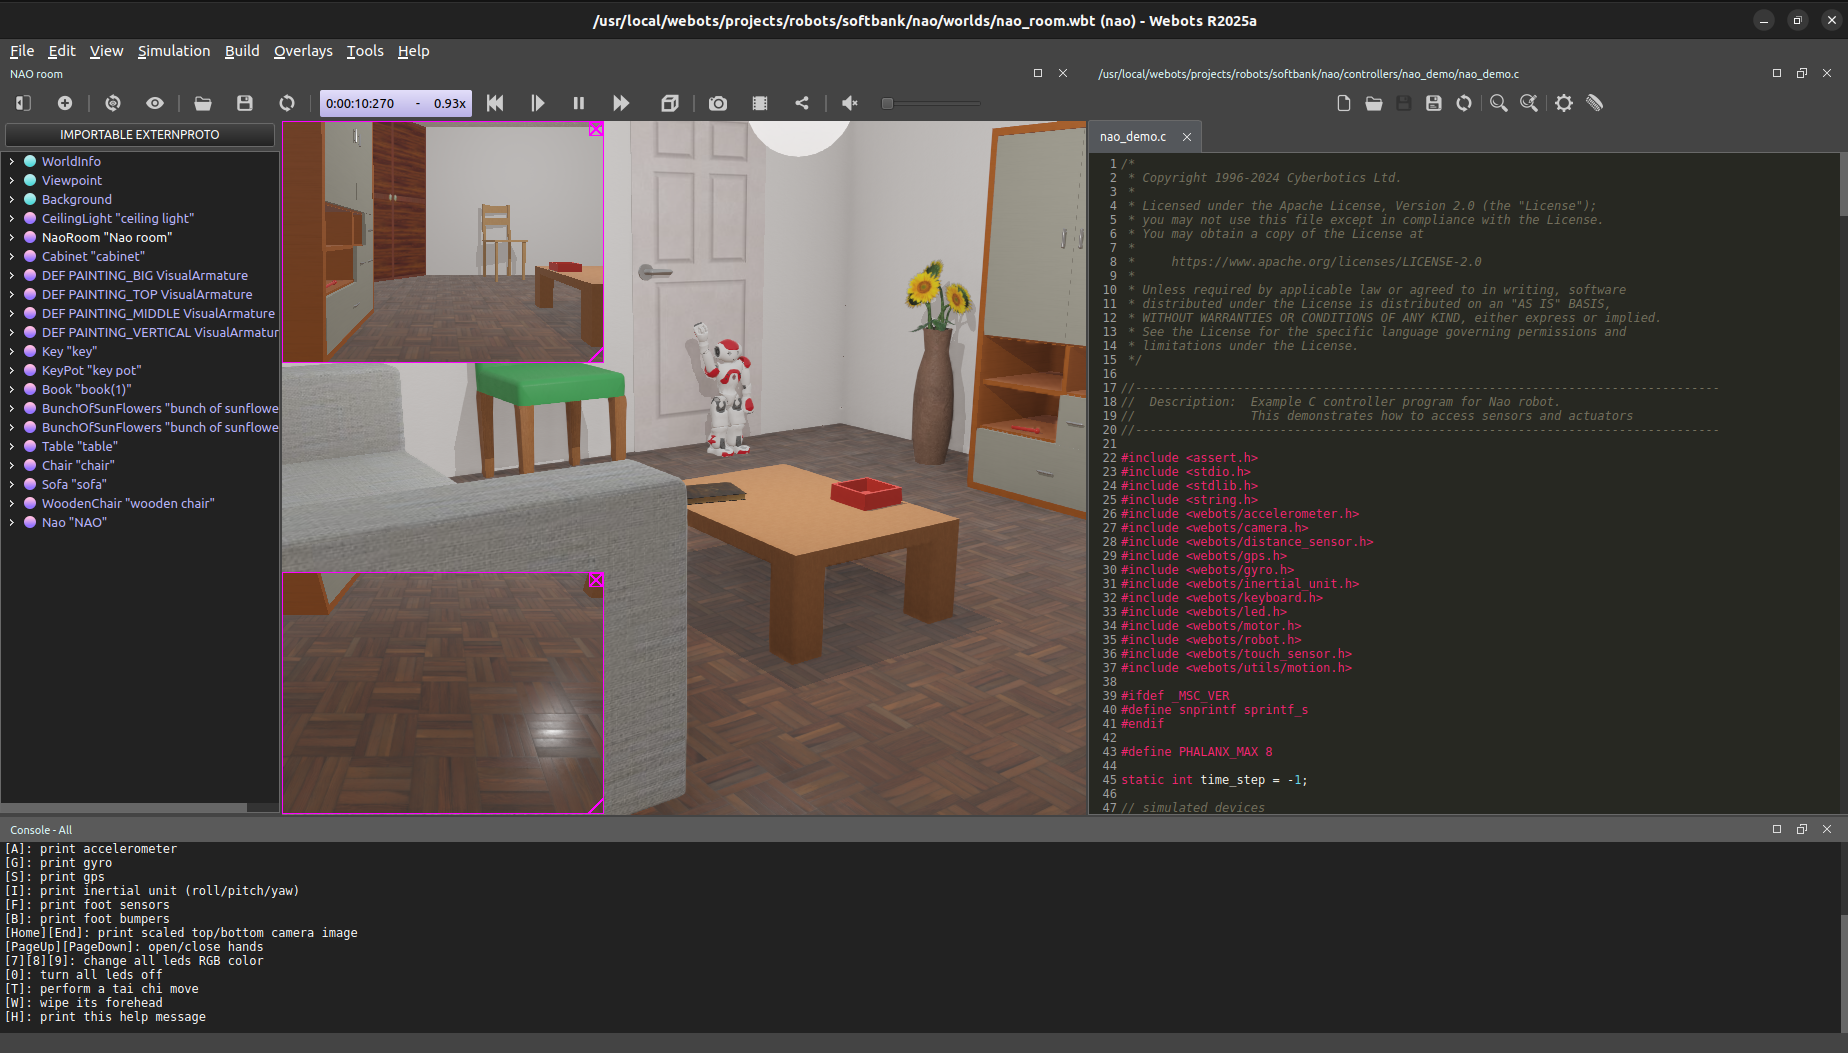
\includegraphics[width=1\textwidth]{figures/cap_3/webots.png}
    \caption{Demo de NAO en Webots}
    \label{fig:demo_webots}
\end{figure}

Se ha utilizado la versión R2025a, que, además de ser la más moderna, ya tiene resueltos patrones de movimiento del robot humanoide NAO que se han reciclado para el desarrollo de este TFG, los cuales son los siguientes:

\begin{itemize}
\item Caminar hacia adelante una secuencia de 10 pasos.
\item Caminar hacia atrás una secuencia de 2 pasos.
\item Levantarse del suelo si se ha caído boca abajo.
\item Caminar de forma lateral una secuencia de 2 pasos hacia la derecha.
\item Caminar de forma lateral una secuencia de 2 pasos hacia la izquierda.
\item Girar en el sitio hacia la derecha un ángulo de 40 grados.
\item Girar en el sitio hacia la derecha un ángulo de 60 grados.
\item Girar en el sitio hacia la izquierda un ángulo de 40 grados.
\item Girar en el sitio hacia la izquierda un ángulo de 60 grados.
\item Girar en el sitio hacia la izquierda un ángulo de 180 grados.
\end{itemize}

El uso de estos patrones y sus modificaciones se extenderá en el Capítulo~\ref{cap:capa_movimiento}.
    \chapter{Capa de movimiento para el humanoide}\label{cap:capa_movimiento}

Una vez explicadas las herramientas utilizadas en el capítulo anterior, en este se explicará el proyecto como tal, desglosando adecuadamente cada una de las partes involucradas en él.

\section{Preparación del modelo} \label{sec:prep_modelo}

Cómo se mencionó en el capítulo \ref{cap:herramientas}, el modelo utilizado fue extraído de la librería abierta de Gazebo.
Sin embargo, este modelo no era suficiente para poder desarrollar todo el proyecto directamente y fue necesario prepararlo y adaptarlo para poder usarlo cómo es debido.

\subsection{Compatibilidad del modelo con ROS2}

Lo primero que se hizo para poder usar el modelo fue preparar los \textit{topics} de ROS2 necesarios para poder publicar posiciones en sus articulaciones y así hacer el modelo compatible con este middleware, ya que como se aprecia en la \autoref{fig:topics_independientes}, tenía los \textit{topics} preparados para Gazebo, y no para ROS. Esto es porque en la versión de Gazebo de 2018, Gazebo Ignition/Gazebo Sim, el simulador se rediseñó desde cero con la idea de ser más independiente de ROS, para que así los usuarios no estuvieran obligados a utilizar dicho middleware para lanzar simulaciones. 

\begin{figure}[H]
  \centering
  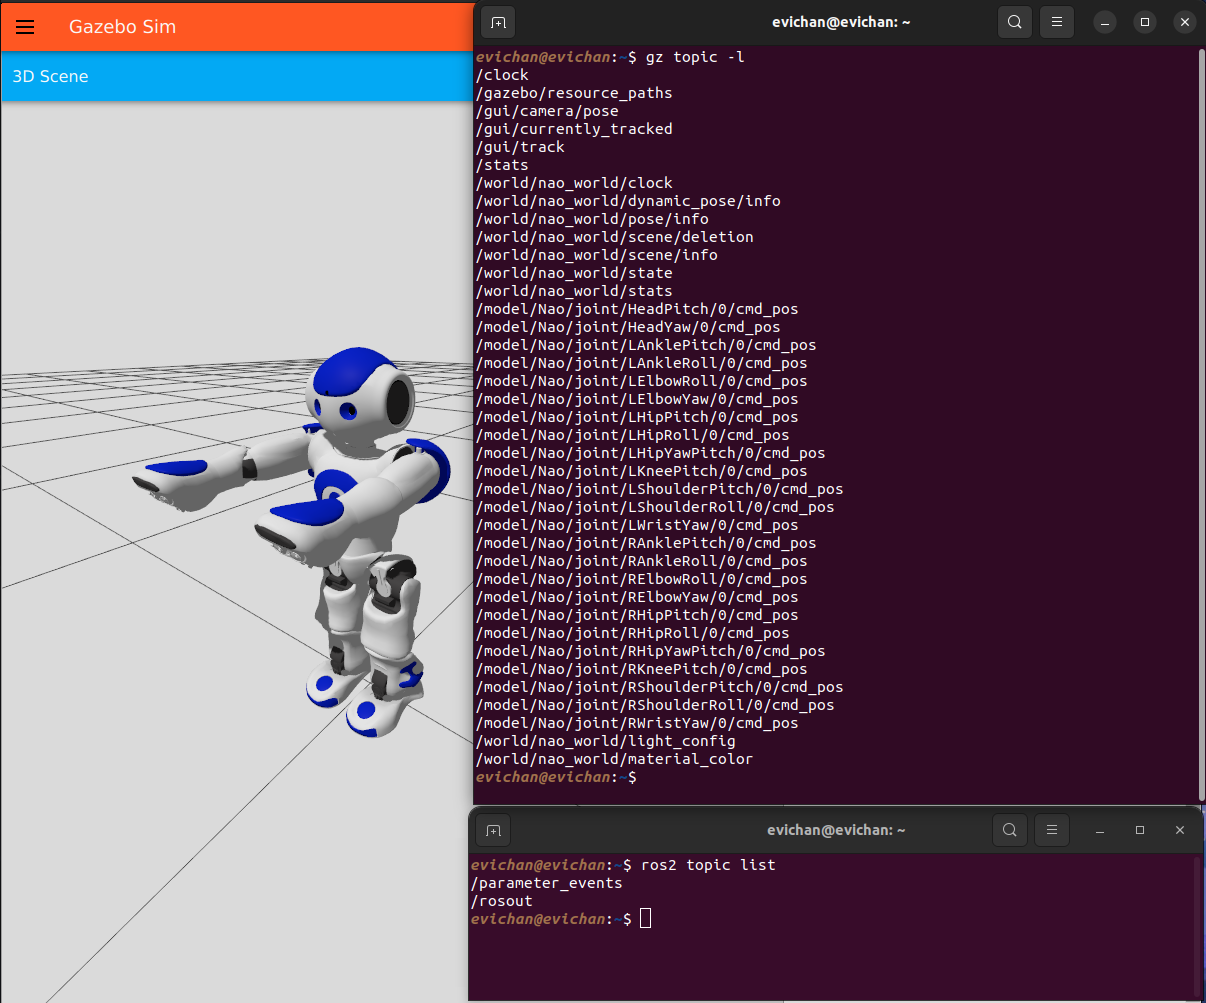
\includegraphics[width=1\textwidth]{figures/cap_4/topics_gazebo.png}
  \caption{\textit{topics} sólo accesibles desde Gazebo y no desde ROS2}
  \label{fig:topics_independientes}
\end{figure}

La solución para este pequeño problema es utilizar un puente que conecta los \textit{topics} de Gazebo con los \textit{topics} de ROS2, disponible en el paquete \textit{ros\_gz\_bridge}\footnote{\url{https://github.com/gazebosim/ros_gz/tree/ros2/ros_gz_bridge}}, que se encarga de que los \textit{topics} de Gazebo sean también visibles al ejecutar el comando \texttt{ros2 topic list}, y no solo al ejecutar \texttt{gz topic -l}, permitiéndonos trabajar con ellos desde ROS2.

Para aplicar este puente, se instala el paquete con \texttt{sudo apt install ros-humble-ros-gz-bridge}. Después, es necesario crear el paquete de ROS que será usado para alojar todos los programas que se iban a lanzar y, además de eso, se debe crear un \textit{launcher.py}, encargado de lanzar la simulación y todos los puentes necesarios para los \textit{topics} de NAO accesibles en Gazebo (todos aquellos que siguen la estructura \textit{/model/NAO/joint/..../0/cmd\_pos}).

Sin embargo, los nombres de los \textit{topics} de Gazebo contienen el número 0 en sus nombres, cosa incompatible con los \textit{topics} de ROS2.

Por lo que, el primer cambio que se tuvo que hacer al modelo fue cambiar el nombre de todos los \textit{topics} relacionados con el movimiento del robot para eliminar este número 0. 

Para ello, en el fichero SDF del robot, primero tenía que localizar dónde se alojaban esos \textit{topics}, cosa que no fue sencilla, ya que el modelo no disponía de una etiqueta \textit{topic} o similar, sino que para poder crear estos \textit{topics}, Gazebo utiliza \textit{plugins}\footnote{\url{https://gazebosim.org/libs/plugin/}}, que son fragmentos de código (generalmente en C++) que se cargan en tiempo de ejecución dentro del simulador para extender o modificar su comportamiento, permitiendo agregar funcionalidades personalizadas a los modelos o mundos.

En el caso de los topics, el plugin responsable se especifica debajo de cada joint (articulación) en el archivo SDF del robot NAO de la forma mostrada en el \autoref{lst:plugin_original}:

\begin{lstlisting}[language=XML, caption={Inclusión del plugin en el modelo}, label={lst:plugin_original}, numbers=left, backgroundcolor=\color{gray!10}]    
<plugin
  filename="ignition-gazebo-joint-position-controller-system"
  name="ignition::gazebo::systems::JointPositionController">
  <joint_name>HeadYaw</joint_name>
  <p_gain>10</p_gain>
  <i_gain>0.1</i_gain>
  <d_gain>0.01</d_gain>
  <i_max>1</i_max>
  <i_min>-1</i_min>
  <cmd_max>1000</cmd_max>
  <cmd_min>-1000</cmd_min>
</plugin>
\end{lstlisting}

En dicho código se especifican todas las condiciones necesarias para que la articulación se comporte como un motor real, incluyendo incluso un controlador PID, con sus ganancias p\_gain, i\_gain y d\_gain, pero, lo importante aquí es que el nombre del \textit{topic} no está definido, y es por eso por lo que se recoge el nombre por defecto. El que incluye el número cero en su nombre.

Para cambiar esto, sólo es necesario añadir la línea \texttt{<topic>nombre\_deseado</topic>} en cualquier lugar de la definición del \textit{plugin}. Una vez hecho esto para todos los \textit{topics}, quedaron como se muestra en la \autoref{fig:topics_independientes_cambiados}:

\begin{figure}[H]
  \centering
  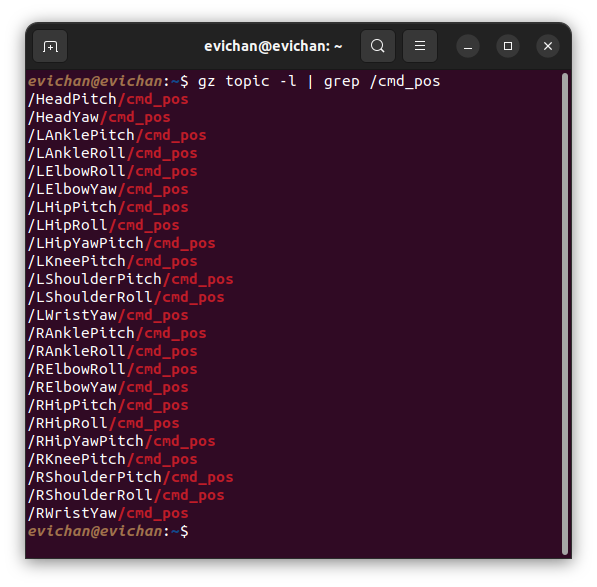
\includegraphics[width=1\textwidth]{figures/cap_4/topics_gazebo_cambiados.png}
  \caption{\textit{topics} corregidos para poder hacer el puente}
  \label{fig:topics_independientes_cambiados}
\end{figure}

Ahora, los \textit{topics} están en el formato correcto para ROS2, por lo que el puente es realizable.

Para crear este puente es necesario incluir en el lanzador del simulador los comandos necesarios para ello. Esto se hace añadiendo las líneas de código que se muestran en el \autoref{lst:estructura_bridge} al \textit{launcher.py} (\cite{tutorial_bridge}):

\begin{lstlisting}[language=Python, caption={Estructura de un \texttt{gz\_bridge}}, label={lst:estructura_bridge}, numbers=left, backgroundcolor=\color{gray!10}]    
gz_bridge_1 = Node(
    package="ros_gz_bridge",
    executable="parameter_bridge",
    name="gz_bridge",
    arguments=[
        "nombre_topic" + "direccion_del_puenteTipo_de_mensaje_ros" + "direccion_del_puenteTipo_de_mensaje_gazebo"
    ],
    output="screen",
)
\end{lstlisting}

Para la dirección del puente, hay que escribir uno de los siguientes símbolos:

\begin{itemize}
  \item \texttt{[:} Puente unidireccional desde Gazebo a ROS. Este puente sólo permite que ROS se suscriba a los \textit{topics}, pero no puede publicar en ellos.
  \item \texttt{]:} Puente unidireccional desde ROS a Gazebo. Este es el caso contrario al anterior, ROS puede publicar, pero no suscribirse.
  \item \texttt{@:} Puente bidireccional. Este puente permite mensajes en ambas direcciones, por lo que ROS puede publicar o suscribirse sin problemas.
\end{itemize}

En este caso, se ha utilizado un puente bidireccional en todos los \textit{topics}, para poder publicar mensajes y suscribirnos a ellos si es necesario.

Para los tipos de mensajes utilizables, es necesario consultar la compatibilidad entre ellos en la tabla\footnote{\url{https://github.com/gazebosim/ros_gz/tree/ros2/ros_gz_bridge/README.md}} dada en el repositorio oficial del paquete \textit{ros\_gz\_bridge}, no sin antes consultar qué tipo tienen nuestros \textit{topics} de Gazebo utilizando el comando \texttt{gz topic -i -t nombre\_del\_topic}.

Una vez definido el tipo de mensajes a utilizar (en nuestro caso, \textit{std\_msgs/msg/Float64 para} ROS y \textit{gz.msgs.Double} para Gazebo), se desarrolló de forma sencilla el launcher del robot con los topics de sus articulaciones compatibles con ROS2. Para ello, se siguió el esquema mostrado en la \autoref{lst:estructura_bridge} y se usaron los componentes necesarios para crear un lanzador adecuado. Un fragmento de dicho \textit{launcher} se ve en el \autoref{lst:launcher}.

\begin{lstlisting}[language=Python, caption={Launcher para simulación sin sensores}, label={lst:launcher}, numbers=left, backgroundcolor=\color{gray!10}]    
#!/usr/bin/env python3
# Importaciones necesarias
def generate_launch_description():
    set_gazebo_version = SetEnvironmentVariable(
        name="GAZEBO_VERSION", value="8.9"
    )
    # Para poder lanzar el mundo
    world_file = PathJoinSubstitution(['/home/evichan/Desktop/2024-tfg-eva-fernandez/GreenNao/greennao/worlds/greenhouse_world', 'greenhouse_world.sdf'])
    declare_world_arg = DeclareLaunchArgument(
        "world", default_value=world_file, description="SDF world file"
    )
    # Para lanzar simulacion de gazebo
    gz_sim = IncludeLaunchDescription(
        PythonLaunchDescriptionSource(
            PathJoinSubstitution(
                [
                get_package_share_directory("ros_gz_sim"),
                    "launch",
                    "gz_sim.launch.py",
                ]
            )
        ),
        launch_arguments={"gz_args": world_file}.items(),
    )
    # Ros bridges para controlar articulaciones de NAO van aqui, uno por grado de libertad
    [...]
    return LaunchDescription(
        [
            declare_world_arg,
            set_gazebo_version,
            SetParameter(name="use_sim_time", value=True),
            gz_sim,
            gz_bridge_1,
            [...] # resto de bridges
        ]
    )
\end{lstlisting}

Una vez ejecutado este \textit{launcher}, además de ver el mundo creado y la simulación completa, podemos ver en la terminal cómo ahora los \textit{topics} se comparten entre ROS2 y Gazebo. Un ejemplo de esto se muestra en la \autoref{fig:topics_ros}.

\begin{figure}[H]
  \centering
  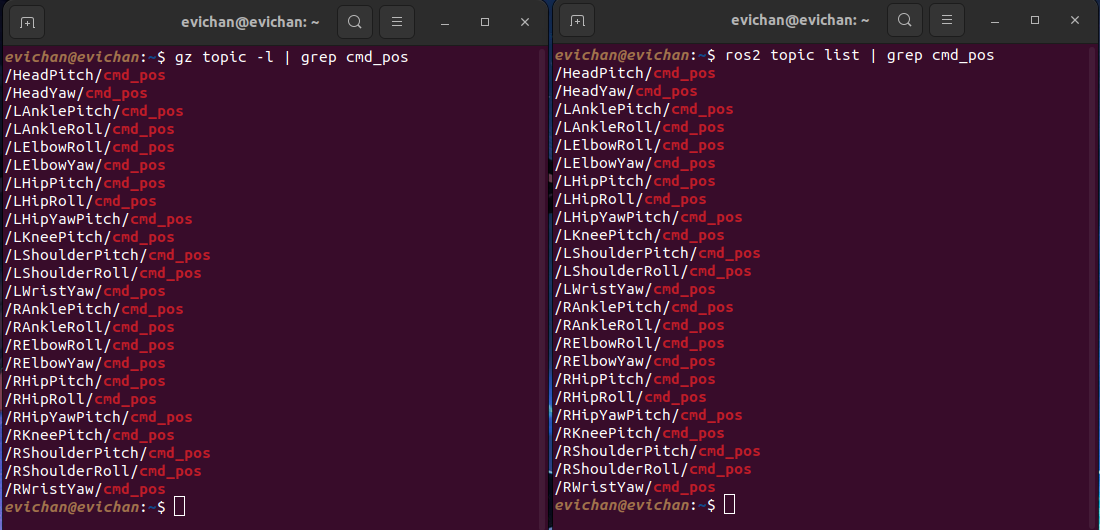
\includegraphics[width=1\textwidth]{figures/cap_4/topics_ros.png}
  \caption{\textit{topics} accesibles desde ROS2 y Gazebo}
  \label{fig:topics_ros}
\end{figure}

\subsection{Adición de sensores}

No sólo fue necesario hacer el modelo compatible con ROS2, sino que también fue  necesario
enriquecer un poco al robot dotándole de sensores, ya que el modelo de Gazebo no los ofrecía. 

Se optó por añadir una cámara y un sensor IMU para que fueran usables en el futuro, además de que son sensores muy utilizados en robótica en general.

\subsubsection{Cámara}
Para añadir una cámara al robot y dotarle de visión, fue necesario insertarle al modelo los campos necesarios para que tuviera una cámara completamente funcional y usable con ROS2, así que, para ello, se añadieron los elementos mostrados en el \autoref{lst:camara_modelo} al SDF del modelo.

\begin{lstlisting}[language=XML, caption={Adición de la cámara al modelo}, label={lst:camara_modelo}, numbers=left, backgroundcolor=\color{gray!10}]   
# Definicion del joint necesario para anclar la camara al torso del robot
[...]
<link name="camera_rgb_frame">
  # Definicion de masa e inercia para en sensor
  [...]
  <sensor name="camera" type="camera">
    <always_on>true</always_on>
    <visualize>true</visualize>
    <update_rate>30</update_rate>
    <topic>NAO/camera/image_raw</topic>
    <gz_frame_id>camera_rgb_frame</gz_frame_id>
    <camera name="intel_realsense_r200">
      <camera_info_topic>NAO/camera/camera_info</camera_info_topic>
      <horizontal_fov>1.02974</horizontal_fov>
      <image>
        <width>1920</width>
        <height>1080</height>
        <format>R8G8B8</format>
      </image>
      <clip>
        <near>0.02</near>
        <far>300</far>
      </clip>
      <noise>
        <type>gaussian</type>
        <mean>0.0</mean>
        <stddev>0.007</stddev>
      </noise>
    </camera> 
  </sensor>
</link>
<plugin filename="gz-sim-sensors-system" name="gz::sim::systems::Sensors">
    <render_engine>ogre2</render_engine>
</plugin>
\end{lstlisting}

\subsubsection{Sensor IMU}
Para que el robot pudiera localizarse utilizando una IMU, fue necesario añadir los siguientes campos al modelo dentro del link del torso:

\begin{lstlisting}[language=XML, caption={Adicición del sensor IMU al modelo}, label={lst:imu_modelo}, numbers=left, backgroundcolor=\color{gray!10}]    
<sensor name="imu_sensor" type="imu">
    <pose>0 0 0 0 0 0</pose>
    <always_on>true</always_on>
    <update_rate>50</update_rate>
    <visualize>true</visualize>
    <topic>NAO/imu_sensor</topic>
    <imu>
    <angular_velocity>
        <noise>
        <type>gaussian</type>
        <mean>0.0</mean>
        <stddev>0.01</stddev>
        </noise>
    </angular_velocity>
    <linear_acceleration>
        <noise>
        <type>gaussian</type>
        <mean>0.0</mean>
        <stddev>0.01</stddev>
        </noise>
    </linear_acceleration>
    </imu>
</sensor>       
</link>
<plugin filename="gz-sim-imu-system" name="gz::sim::systems::Imu">
    <topic>NAO/imu_sensor</topic>
</plugin> 
\end{lstlisting}

Después de añadir estos sensores al SDF del modelo, se añadieron también los puentes necesarios al \textit{launcher} para que ROS pudiera acceder a sus lecturas, de la misma forma vista anteriormente en el \autoref{lst:launcher}.

Una vez los sensores fueron añadidos correctamente, los \textit{topics} finales del robot eran los siguientes:

\begin{figure}[H]
  \centering
  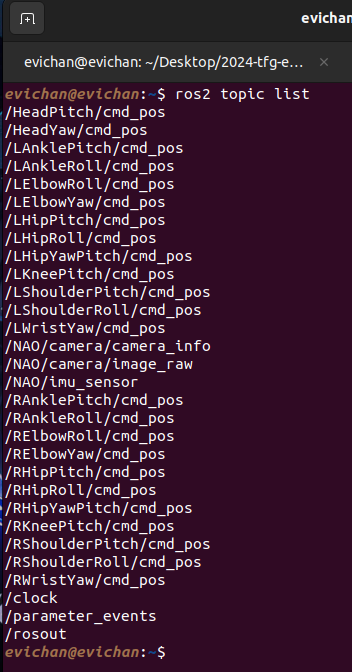
\includegraphics[width=0.5\textwidth]{figures/cap_4/topics_completos.png}
  \caption{\textit{topics} finales del robot}
  \label{fig:topics_completos}
\end{figure}

\subsection{Estabilidad estática}

Un problema que tienen los robots humanoides, como se comentaba en el capítulo \ref{cap:introduccion}, es que tienen que ser estables tanto dinámica cómo estáticamente, el NAO no es una excepción.

Cuando introduje al robot en el mundo por primera vez, éste caía de boca al suelo, cosa que indicaba que el modelo no era estáticamente estable.

Para dotarle de esta estabilidad, se compensó el peso del humanoide con las posiciones iniciales de sus articulaciones y su posición inicial, a base prueba y error.

Cambiar la posición inicial no tiene ningún misterio, ya que simplemente es cambiar el campo \textit{pose} que está al incio del modelo. Sin embargo, las posiciones iniciales de las articulaciones tuvieron más complicación.

Para asignarlas, tuve que añadir los campos \texttt{<initial\_position>} y \texttt{<use\_velocity\_commands>true</use\_velocity\_commands>}, seguido de los campos \texttt{cmd\_max} y \texttt{cmd\_min} al plugin de las articulaciones para que la velocidad no fuera demasiado brusca para el movimiento y la articulación se moviera correctamente a la posición deseada al comienzo de la simulación. Adjunto a continuación un ejemplo de estos cambios (\autoref{lst:ejemplo_posicion_inicial}), y un vídeo\footnote{\url{https://drive.google.com/file/d/12jZqSiFHvwvEwgq3LtMei6cYimbpxVOT/view?usp=sharing}} del resultado final de este cambio.  

\begin{lstlisting}[language=XML, caption={Ejemplo de configuración de posición inicial de una articulación}, label={lst:ejemplo_posicion_inicial}, numbers=left, backgroundcolor=\color{gray!10}]    
<plugin filename="ignition-gazebo-joint-position-controller-system" name="ignition::gazebo::systems::JointPositionController">
    [...]
    <use_velocity_commands>true</use_velocity_commands>
    <cmd_max>2.0</cmd_max>
    <cmd_min>-2.0</cmd_min>
    [...]
    <initial_position>1.39626</initial_position>
</plugin>
\end{lstlisting}

Por tanto, para lograr esta estabilidad estática, el robot debe comenzar con las siguientes posiciones:

\begin{itemize}
  \item Posición inicial del robot: x=0 y=0 z=0.5 rx=0 ry=0.240818894505798 rx=0
  \item /HeadPitch/cmd\_pos: 0
  \item /HeadYaw/cmd\_pos: 0
  \item /LAnklePitch/cmd\_pos: -0.479
  \item /LAnkleRoll/cmd\_pos: 0
  \item /LElbowRoll/cmd\_pos: -1.0472
  \item /LElbowYaw/cmd\_pos: -1.39626
  \item /LHipPitch/cmd\_pos: -0.179
  \item /LHipRoll/cmd\_pos: 0
  \item /LHipYawPitch/cmd\_pos: 0
  \item /LKneePitch/cmd\_pos: 0.698132
  \item /LShoulderPitch/cmd\_pos: 1.39626
  \item /LShoulderRoll/cmd\_pos: 0.198132
  \item /LWristYaw/cmd\_pos: -0.192
  \item /RAnklePitch/cmd\_pos: -0.479
  \item /RAnkleRoll/cmd\_pos: 0
  \item /RElbowRoll/cmd\_pos: 1.0472
  \item /RElbowYaw/cmd\_pos: 1.39626
  \item /RHipPitch/cmd\_pos: -0.179
  \item /RHipRoll/cmd\_pos: 0
  \item /RHipYawPitch/cmd\_pos: 0
  \item /RKneePitch/cmd\_pos: 0.698132
  \item /RShoulderPitch/cmd\_pos: 1.39626
  \item /RShoulderRoll/cmd\_pos: -0.198132
  \item /RWristYaw/cmd\_pos: 0.192
\end{itemize}

También fue necesario editar el peso de ambos pies, ya que el robot tenía más peso en el tren superior que en el inferior y esto le impedía levantarse, así que se sumó 1 de peso a cada pie y se modificaron sus matrices de inercia para adaptarlos correctamente a su nueva masa.

\subsection{Retoque estético}

Cómo último preparativo del modelo, se editó su textura para que tuviera un color distinto, así se lograría dar un poco de identidad al modelo y, de cara a la aplicación final, que fuera más vistoso.

El resultado de este retoque se puede ver en la \autoref{fig:nao_retocado}.

\begin{figure}[H]
  \centering
  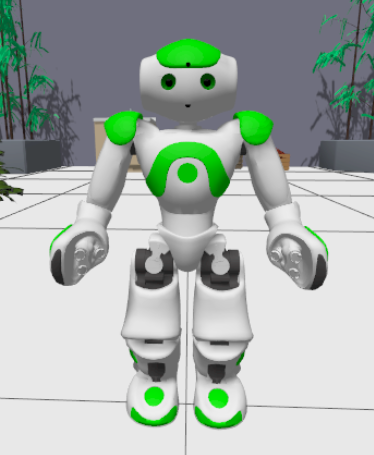
\includegraphics[width=0.5\textwidth]{figures/cap_4/GreenNao.png}
  \caption{Nao retocado estéticamente}
  \label{fig:nao_retocado}
\end{figure}

Una vez terminadas estas modificaciones, el modelo estaba completamente preparado, ya era posible su programación, y por ende el desarrollo del proyecto como tal.

\section{Editor e intérprete de movimientos}

El primer elemento clave de este proyecto es el editor de movimientos, una herramienta capaz de crear patrones fijos de movimiento para coordinar las articulaciones de NAO de forma cómoda.

Aunque, una vez creados estos patrones, también es necesario crear un intérprete que permita a NAO replicar los patrones creados, también de forma cómoda. Es por esto que editor e intérprete van de la mano y se describen a continuación.

\subsection{Editor} \label{subsec:editor}

Este editor consiste en un programa que permite al usuario crear patrones de movimiento para que posteriormente sean interpretados por el intérprete y a su vez replicados por el robot. Está basado en \textit{KME} (\cite{paper_1},\cite{paper_2}), un editor de movimientos basado en fotogramas clave (\textit{keyframes}). Permite al usuario crear secuencias de posiciones para cada articulación del robot en momentos específicos del tiempo. Es especialmente útil para programar movimientos complejos y sincronizados, como saludar o tomar una pose concreta, siendo estos patrones siempre fijos y no modificables a a hora de interpretarse.

El programa se ha desarrollado en Pyhton, y utiliza el simulador Pybullet\footnote{\url{https://Pybullet.org/wordpress/index.php/forum-2/}} para poder ofrecer al usuario una visión directa del NAO y sus movimientos a la hora de crear el patrón.

Para que todo funcionase correctamente en Pybullet, era necesario tener disponible al modelo de NAO, para cumplir la parte de la visualización en tiempo real de los movimientos.

Sin embargo, el formato SDF del modelo que se preparó no es compatible con Pybullet, siendo el formato necesario URDF. Por suerte, se encontró un modelo de NAO en URDF disponible para descargar en un repositorio público de github\footnote{\url{https://github.com/ros-naoqi/nao_robot/blob/master/nao_description/urdf/naoV40_generated_urdf/nao.urdf}}. También fue necesario modificar este URDF para que fuera lo más igual posible al modelo en SDF, esto es, ponerle las posiciones iniciales de las articulaciones (cosa que se hace directamente en el código del editor), editar los pesos de los pies para que fueran iguales a los del SDF, ajustar los límites de las articulaciones, etc. 

La aplicación del editor es capaz de conectarse a los joints de NAO gracias a Pybullet, que dispone de una API específica para hacerlo, por lo que, es necesario tener en cuenta todos los \textit{topics} (articulaciones) que se iban a manejar y qué movimientos y grados de libertad tenemos disponibles, para eso es muy útil el esquema mostrado en la \autoref{fig:esquema_joints}:

\begin{figure}[H]
  \centering
  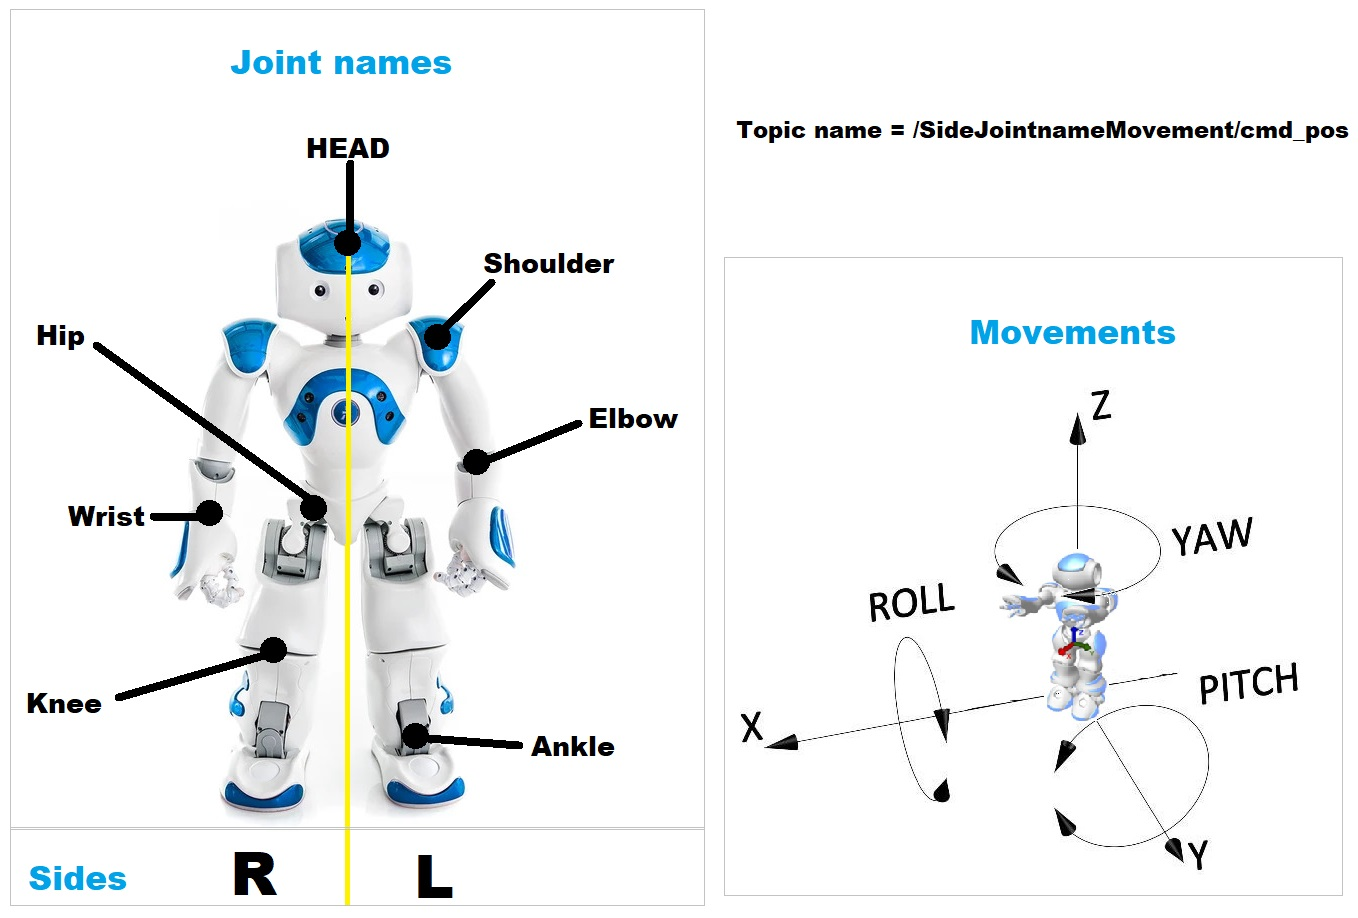
\includegraphics[width=1\textwidth]{figures/cap_4/esquema_joints_NAO.jpeg}
  \caption{Esquema de \textit{topics} y articulaciones de NAO}
  \label{fig:esquema_joints}
\end{figure}

Cómo se puede ver, este robot ofrece mucha variedad de movimientos, con un total de 24 grados de libertad.

Para controlar cada uno de ellos en Pybullet de forma cómoda, se ofrece una interfaz con barras deslizantes o \textit{sliders} para que el manejo sea más visual y fácil de abarcar, esto es porque las articulaciones tienen un límite y no todas las posiciones son válidas. Con estas barras el usuario puede ver fácilmente dichos límites.

Este sistema de \textit{sliders} lo ofrece Pybullet de forma cómoda, simplemente escribiendo lo mostrado en el \autoref{lst:ejemplo_slider} en el código del editor:

\begin{lstlisting}[language=Python, caption={Ejemplo de adicición de sliders al editor}, label={lst:ejemplo_slider}, numbers=left, 
backgroundcolor=\color{gray!10}]    

# Preparar el slider
joint_slider = p.addUserDebugParameter("nombre del joint", minimo, maximo, posicion inicial)

# Dentro del bucle principal (omitido ahora) Lectura del slider
joint_value = p.readUserDebugParameter(joint_slider)

# Ejecucion del movimiento en el modelo
p.setJointMotorControl2(model,1, p.POSITION_CONTROL, targetPosition=joint_value, maxVelocity=2)
\end{lstlisting}

Con esto para cada una de las articulaciones, somos capaces de controlar íntegramente a NAO, aún sin posibilidad de guardar los movimientos deseados.

Para esto se han utilizado ficheros JSON, de modo que se han añadido 2 sliders adicionales, uno para indicar el tiempo en el que se desea adoptar esa posición (tiempo del fotograma), y otro más que indica al programa que se quiere guardar el patrón, el cual, cuando cambia de posición, guarda automáticamente el fichero y avisa al usuario.

Un ejemplo del formato que tienen estos ficheros JSON se muestra en el \autoref{lst:ejemplo_json}.

\begin{lstlisting}[language=, caption={Ejemplo de JSON}, label={lst:ejemplo_json}, numbers=left, 
backgroundcolor=\color{gray!10}]    
[
    {
        "tiempo": 1,
        "articulaciones": [
            {
                "articulacion": "HeadYaw",
                "posicion": 2.0901734911206137e-08
            },
            [...] # resto de articulaciones
        ]
    }
]
\end{lstlisting}

Se adjunta un enlace a un vídeo\footnote{\url{https://drive.google.com/file/d/1qmmINis9zI1dkMiPdKbTRGS3bIWH4zAP/view?usp=sharing}} demostrativo del funcionamiento de este programa. Cabe destacar que se deja caer al robot al inicio del programa para que el usuario vea que efectivamente hay movimientos y físicas realistas involucrados en él.

\subsection{Intérprete} \label{subsec:interprete}

El editor no resulta muy útil sin que el robot NAO simulado replique los patrones de movimiento creados.

Es por eso por lo que existe el intérprete de movimientos. Este programa consiste en un nodo ROS2 programado en Python que lee los datos del fichero JSON que se le indica por argumento, y se encarga de hacer las publicaciones a los \textit{topics} necesarios en el momento adecuado (replica cada fotograma en la marca de tiempo especificada).

También el usuario podría querer utilizar otros formatos, como el .motion, ofrecido por el simulador Webots\footnote{\url{https://cyberbotics.com/}}. Además, muchos patrones de movimiento ofrecidos en esta aplicación se han conseguido de los ficheros de este simulador, cosa que se explicará con detalle en la seguiente sección y se ha introducido en el capítulo \ref{cap:herramientas}.

Como Python no ofrece soporte para leer este tipo de ficheros directamente, se optó por adpatarlos a formato CSV y después añadir también al nodo intérprete la posibilidad de leer este tipo de ficheros.

Para hacer este nodo, se ha utilizado una calidad de servicio como la que se muestra en el \autoref{lst:calidad_de_servicio} para evitar la fatiga a la hora de publicar varios mensajes, ya que estaremos casi constantemente publicando mensajes en cada articulación.

\begin{lstlisting}[language=Python, caption={Calidad de servicio utilizada para publicación de mensajes}, label={lst:calidad_de_servicio}, numbers=left, backgroundcolor=\color{gray!10}]    
qos_profile = QoSProfile(
            reliability=ReliabilityPolicy.RELIABLE,
            history=HistoryPolicy.KEEP_ALL,
            depth=100
)
\end{lstlisting}
 
A continuación, se adjunta un vídeo\footnote{\url{https://drive.google.com/file/d/1Uu_XeUeyez8WDv1lKX4hO-0H0RXsXJr1/view?usp=sharing}} demostrativo de este intérprete de movimientos.

Este intérprete evoluciona a una función dentro de la librería que se ha desarrollado para encapsular el uso de ROS2, por lo que dejará de utilizarse como nodo independiente. 

\section{Librería} \label{sec:librería}

En cuanto a la librería desarrollada, ésta se encarga de que el uso de ROS2 sea parcialmente transparente para el usuario, ya que su instalación y uso básico (creación de un paquete para utilizarla, compilarlo, etc) sigue siendo necesario.

Para conseguir este encapsulamiento, es necesario que la librería contenga los nodos a utilizar (clases de python que se encargan de la publicación de las posiciones a las articulaciones) y una función que active estos nodos, que corresponde a la llamada por el usuario.

Para poder activar los nodos, se requiere el uso de rclpy\footnote{\url{https://docs.ros.org/en/rolling/p/rclpy/}}, que proporciona la API canónica de Python para interactuar con ROS2.

Un ejemplo de cómo han de crearse estas clases para que los nodos funcionen correctamente se muestra en el \autoref{lst:funcion_rclpy}.

\begin{lstlisting}[language=Python, caption={Ejemplo de función que invoca un nodo ROS2}, label={lst:funcion_rclpy}, numbers=left, backgroundcolor=\color{gray!10}]    
def Interpreter(file_name: str, printable=True):
    rclpy.init()
    node = Interpreter_class(file_name, printable)
    
    try:
        rclpy.spin_once(node, timeout_sec=2)
    
    finally:
      node.destroy_node()
      rclpy.shutdown()
\end{lstlisting}

Hay 3 tipos de estas funciones, las que sirven para llamar a nodos cuya tarea es replicar patrones fijos creados con el intérprete; las que sirven para invocar a nodos capaces de replicar movimientos parametrizables y las que sirven para leer los sensores.

\subsection{Primer tipo de funciones: Patrones fijos}

El primer tipo de función es la evolución del nodo intérprete de movimientos que se explicó en la sección \ref{subsec:interprete}, que hace que pase de nodo independiente de ROS2 a función de esta librería.

El nombre de la función es \textit{Interpreter} (mostrada en la \autoref{lst:funcion_rclpy}) y recibe como argumento el nombre del fichero a replicar como \textit{string} y el parámetro opcional boolenao \textit{printable}, que indica si es necesario o no imprimir un \textit{log} final. Este parámetro es utilizado por todos los nodos y funciones que se llaman desde otras funciones, para que cada una tenga sus \textit{logs} por separado. 

Un ejemplo de esto sería una función que llame a este intérprete, llamada hipotéticamente \textit{función}, la cual tiene un \textit{log} final como este: \texttt{[Función]: Mensaje final}. Sin el parámetro \textit{printable}, se imprimirían el \textit{log} final de la función del intérprete (\texttt{[Intepreter]: Movimientos de fichero fichero.json completados}) y después el de la función anteriormente mencionada, lo que podría llevar a confusión al usuario por ver nombres de funciones que puede no haber llamado explícitamente.

Si este parámetro \textit{printable} se pasa como  verdadero, el \textit{log} se imprimirá, lo contrario ocurriría si el parámetro toma el valor de falso. Si no se le pasa (al ser este un parámetro opcional), su valor predeterminado es \textit{True}.

El nodo al que llama esta función se encarga de leer e fichero epecificado, crear un publicador para cada aticulación que aparezca en el fichero y publicar en el tiempo especificado la posición idicada para  cada articulación, consiguiendo así una secuencia estable de fotogramas. Su funcionamiento es el mismo que el explicado en la sección \ref{subsec:interprete}, incluida la calidad de servicio.

También a este tipo de funciones pertenecen las siguientes:

\begin{itemize}
    \item \textit{wakeup\_face\_down}: Esta función no recibe parámetros y se encarga de llamar al intérprete las veces necesarias para ejecutar el patrón de levantar al robot del suelo en caso de haber caído boca abajo o de \textit{cubito prono}. Este patrón fue recogido del simulador Webots.
    \item \textit{wakeup\_face\_up}: Esta función no recibe parámetros y se encarga de llamar al intérprete las veces necesarias para ejecutar el patrón de levantar al robot del suelo en caso de haber caído boca arriba o de \textit{cubito supino}. Este patrón consiste en que nao se de la vuelta (patrón creado con el editor en formato JSON), y depués ejecutar el patrón que lo levanta desde \textit{cubito prono}
    \item \textit{stand\_still}: Esta función recibe el parámetro opcional \textit{printable} y sirve para que NAO adopte la postura predeterminada explicada en la sección \ref{sec:prep_modelo} llamando al intérprete con el fichero que indica esta posición, creado con el editor en fomato JSON.
    \item \textit{say\_hi}: Esta función toma como parámetro la \textit{string hand}, que puede tomar los valores L, left, LEFT, R, right o RIGHT, que sirve para indicar a NAO con qué mano debe saludar llamando al intérprete con el fichero adecuado. Los patrones para ambas manos fueron creados con el editor enn formato JSON.  
    \item \textit{turn}: Esta función toma como parámetro una \textit{string} que puede tomar como valores los mismos que la función \textit{say\_hi} y un entero que puede tomar los valores 40, 60 o 180, siendo este último posible sólamente en el caso de que la string indique el lado izquierdo, ya que esta función se encarga de que el intérprete llame a los patrones de giro en el sitio adecuados, rescatados de webots, el número indica los grados a girar. También recibe el parámetro opcional \textit{printable}.
    \item \textit{grab\_box}: Esta función no recibe parámetros y se encarga de que el intérprete lance el patrón necesario para coger una caja, creado con el editor en formato JSON. Esta función será útil para la aplicación propuesta.
    \item \textit{release\_box}: Esta función no recibe parámetros y es análoga a la anterior, ya que es igual, pero el patrón es para dejar la caja recogida. Patrón también creado con el editor e formato JSON.
\end{itemize}

Se pueden ver vídeos demostrativos de todas estas funciones en el siguiente enlace\footnote{\url{https://drive.google.com/drive/folders/1s-uI7KXyk6aZ8lbhQIRRZnR8VsfDIsj6?usp=sharing}}.

\subsection{Segundo tipo de funciones: Patrones parametrizables}

Estas funciones son más complejas que las anteriores, ya que cada una de ellas debe ser capaz de ``editar'' el patrón requerido en función del parámetro facilitado.

En el caso de este TFG, y porque para los modos de caminar es necesario (sin ellos no se podría llevar a cabo ninguna aplicación útil para NAO), se ha optado por parametrizar la velocidad de los movimientos, en este caso los pasos.

Todas las funciones de este tipo se encargan de modos de caminar para el humanoide, y hacen que la caminata sea más rápida o más lenta.

La manera de poder parametrizar este valor de la velocidad es modificando los tiempos del fotograma, de esta forma, si el tiempo aumenta, el movimiento será más lento, si disminuye, será más veloz.

Para que este parámetro tuviera una interfaz sencilla, se ha seguido el esquema mostrado en la \autoref{fig:vel_value} a la hora de parametrizarlo.

\begin{figure}[H]
  \centering
  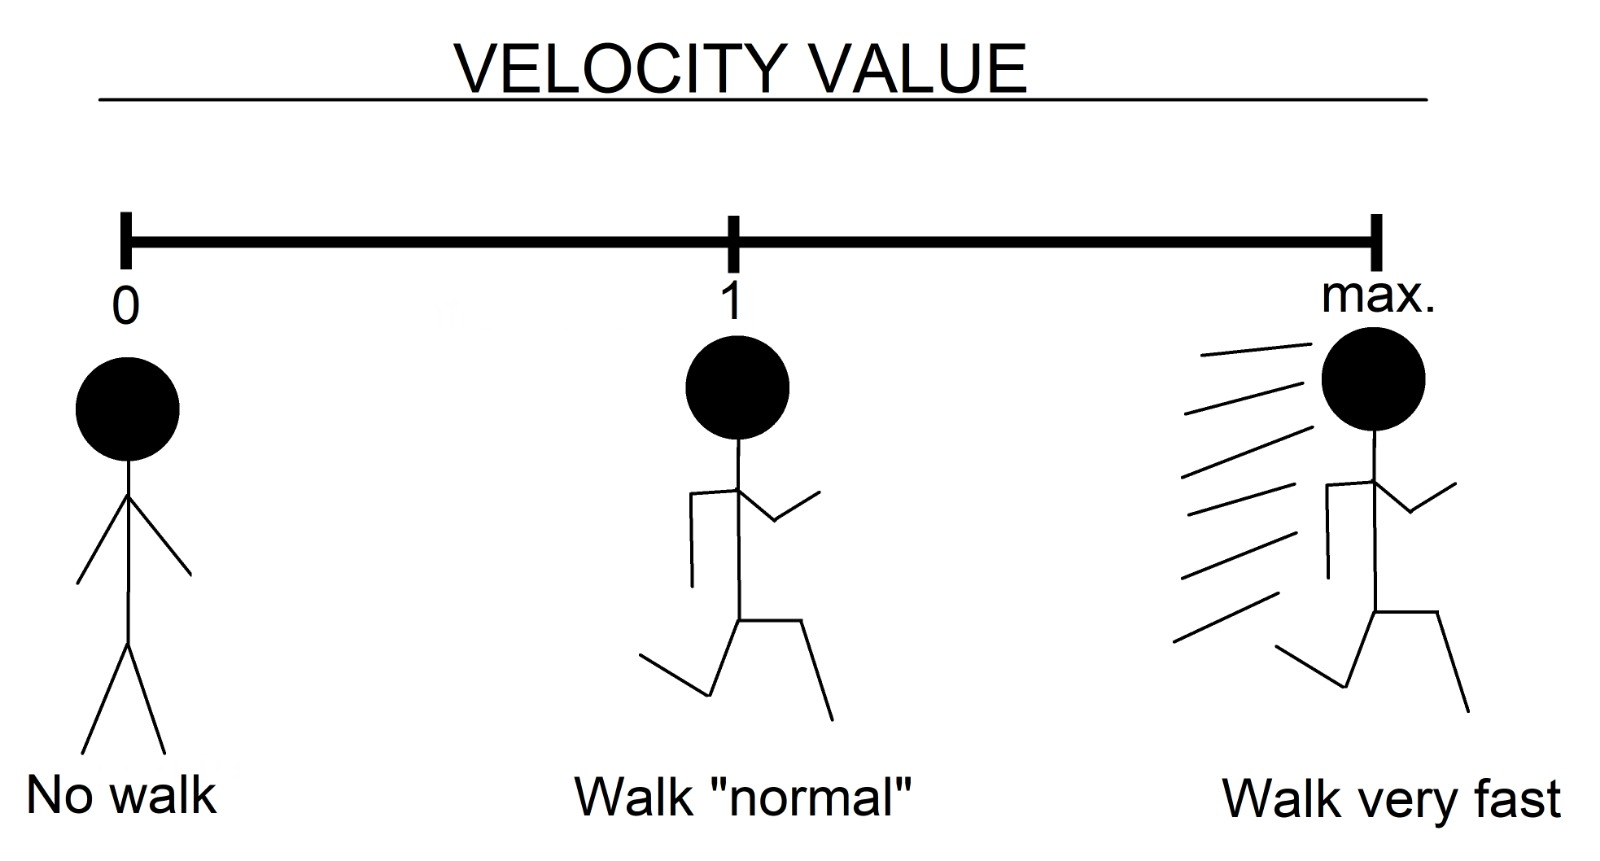
\includegraphics[width=1\textwidth]{figures/cap_4/velocity_value.jpeg}
  \caption{Esquema de parametrización de la velocidad}
  \label{fig:vel_value}
\end{figure}

Para conseguir este efecto, ha sido necesario dividir el tiempo de cada fotograma entre el parámetro de velocidad introducido, de esta manera, se consigue que cuando el parámetro sea menor que 1, el tiempo aumente, y lo contrario en caso de que el parámetro sea mayor que 1. Así también nos aseguramos de que el parámetro quede ``predeterminado'' si le pasamos velocidad igual a 1.

Sin embargo, se debe tener precaución a la hora de pasar este parámetro, ya que una velocidad demasiado baja hará que los fotogramas no vayan con la fluidez mínima requerida y el robot se mueva de manera poco realista, dejando demasiado espacio temporal entre un fotograma y el siguiente. De forma análoga, una velocidad demasiado alta provocará inestabilidad absoluta en la caminata, y los fotogramas siguientes ``atropellarán'' a los anteriores, haciendo que el robot caiga.

Para evitar que el usuario utilice valores inadecuados, cada una de estas funciones cuenta con un valor mínimo y uno máximo permitidos. Estos límites se especificarán en la explicación correspondiente de cada función, presentada más adelante.

Esta velocidad puede ser lineal, angular o lateral y tomar valores positivos y negativos, siguiendo estas normas:
\begin{itemize}
    \item \textit{Velocidad positiva}: Implica movimientos hacia adelante o a la derecha, dependiendo de si la velocidad es lineal o angular/lateral.
    \item \textit{Velocidad negativa}: Implica movimientos hacia atrás o la izquierda, dependiendo de si la velocidad es lineal o angular/lateral.
\end{itemize}

Este efecto se logra gracias a que hay patrones para ambas direcciones, y dependiendo del caso se utiliza uno u otro.

Cabe destacar que no sólo se ha parametrizado la velocidad, también se ha parametrizado el número de pasos que el robot puede dar. Este mínimo viene dado por el patrón predeterminado en formato CSV y puede ser 10 o 2, dependiendo del caso. Para parametrizarlo, simplemente se repite en un bucle \textit{for} el patrón \texttt{pasos\_indicados/mínimo} veces, por lo que el parámetro de los pasos también debe ser múltiplo del mínimo. Dicho valor mínimo también se detallará a continuación.

Cada una de estas funciones son como la mostrada en la \autoref{lst:funcion_rclpy}, debido a que estos patrones se logran mediante nodos ROS2 que deben ser invocados.

Estas funciones son las siguientes:
\begin{itemize}
    \item \textit{setL}: Esta función tiene como objetivo que NAO se desplace lateralmente (utilizando velocidad lateral). Los patrones utilizados se han recogido de webots y tiene un mínimo de 2 pasos, con velocidad mínima de -0.35 ó 0.35, dependiendo de la dorección a la que se quiera avanzar y una máxima de 4.35 ó -4.35. 
    \item \textit{setV}: Esta función se encarga de hacer al robot caminar en linea recta (utilizando velocidad lineal), el mínimo de pasos en este caso es algo especial, ya que, si se le pasa velocidad negativa, el patrón sólo tiene 2 pasos, por lo que en este caso, el bucle se repite \textit{5*pasos\_indicados}, para que el número de pasos aplique a ambos patrones, ya que el patrón de caminata haia adelante tiene un mínimo de 10 y así ambos lo comparten. Ambos fueron recogidos de webots y los máximos y mínimos de velocidad son los mismos que para la función setL.
    \item \textit{turnVel}: Esta función sirve para que el robot sea capaz de girar en el sitio con velocidad angular parametrizada. Ambos patrones utilizados son recogidos de webots, tienen un mínimo de 10 pasos y unas velocidades de 0.35 y -0.35 para el mínimo, y 1.9 y -1.9 para el máximo.
    \item \textit{setW}: Esta función se encarga de mover a NAO describiendo una trayectoria de arco, sus parámetros son los mismos que la función anterior. Los patrones utilizados fueron creados a base de editar el patrón CSV de la caminata hacia adelante.
    \item \textit{setNW}: Esta función es igual que la anterior, pero los arcos decritos son hacia atrás. LOs patrones utilizados fueron creados a base de editar el patrón CSV de la caminata hacia atrás.
\end{itemize}

Pero, estas funciones por sí solas no representan una forma intuitiva de hacer que el robot camine, por lo que es necesaria una sexta función que encapsule todas estas (excepto la de setL, ya que esa es un modo de caminar más específico y se deja fuera) en una sola con una interfaz amigable para el usuario.

Esta es la función \textit{setArc}, que recibe todos los parámetros necesarios para cada función explicada anteriormente (número de pasos, velocidad, y el parámetro opcional \textit{printable}) para después llamarlas en función de los parámetros recibidos.

Para facilitar la comprensión de esta función, se incluye un esquema que muestra su impacto en la trayectoria del NAO en la \autoref{fig:setarc_esq}.

\begin{figure}[H]
  \centering
  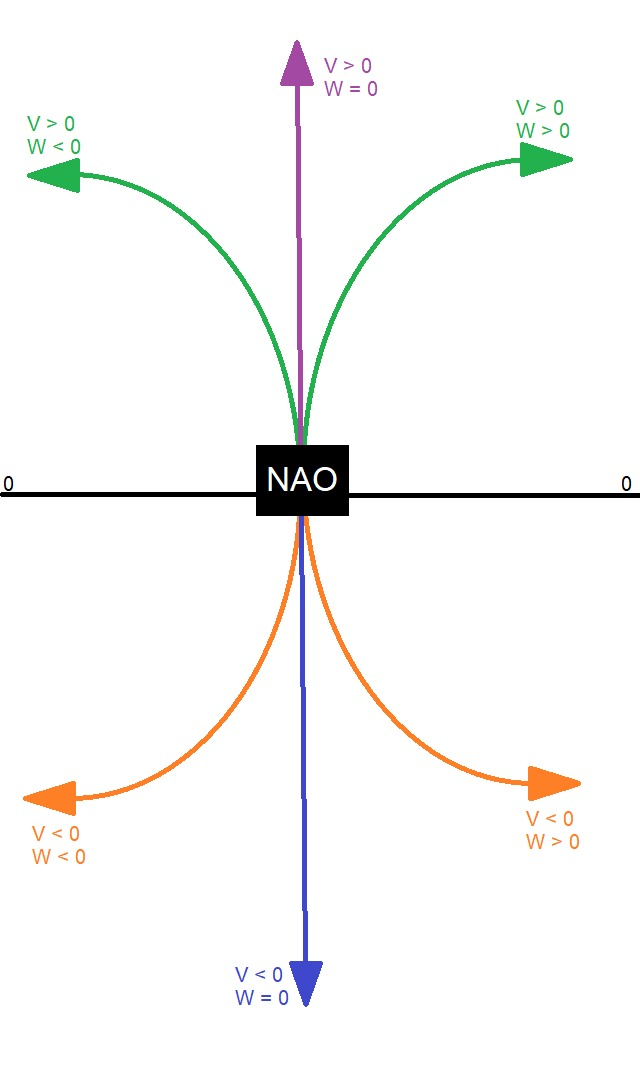
\includegraphics[height=0.8\textwidth]{figures/cap_4/esquema_movs.jpeg}
  \caption{Esquema de funcionamiento de la función setArc}
  \label{fig:setarc_esq}
\end{figure}

El código de esta función tan importante y sencilla al mismo tiempo se encuentra en el \autoref{lst:setarc}
\begin{lstlisting}[language=Python, caption={Función setArc}, label={lst:setarc}, numbers=left, backgroundcolor=\color{gray!10}]    
def setArc(v,w,steps = 10):
    if (not ((0.35 <= abs(w) <= 1.9) or abs(w) == 0) or not (2 <= steps) or (steps%2 != 0)) or (not ((0.35 <= abs(v) <= 4.35) or abs(v) == 0) or not (10 <= steps) or (steps%10 != 0)):
        print("[setArc]: ERROR: La velocidad lineal debe estar entre +-0.35 y +-4.35 y la angular entre +-0.35 y +-1.9, y los pasos deben ser multiplos de 10")
        sys.exit(1)

    if v != 0 and w == 0:
        setV(v, steps, False)

    elif v != 0 and  w != 0:
        if v > 0: 
            setW(w, steps, False)
        else:
            setNW(w, steps, False)
    
    elif v == 0 and w != 0:
        turnVel(w, steps, False)
    
    elif v == 0 and w == 0:
        stand_still(False)

    else:
        print("[setArc] ERROR: Patron de movimiento no valido")
        sys.exit(1)
    
    print("[setArc]: Pasos completados")
\end{lstlisting}

Un video demostrativo que muestra el funcionamiento de las funciones setL, setV y setW está disponible en el siguiente enlace\footnote{\url{https://drive.google.com/drive/folders/15G_RUEmvvaGzpb4Y5p0CmH2KngV0ZB9F?usp=sharing}}, las otras no se adjuntan por ser deriavdas de las demás y funcionar igual o muy parecido.

\subsection{Tercer tipo de funciones: Sensores} \label{subsec:sensores}

También existen funciones cuya misión es leer los datos sensoriales y brindar información al respecto.

Este es el caso de las funciones \textit{Read\_IMU} y \textit{get\_face}.

La primera de las funciones se encarga de devolver la aceleración en z que está experimentando el robot, para que después \textit{get\_face} la recoja y nos indique, en el caso de caída, si NAO está de \textit{cubito supino, cubito prono} o en una posición indeterminada.

Esto nos sirve para saber a qué patrón fijo de levantarse debemos llamar.

En el caso de la cámara, no se ha implementado una función concreta para utlizarla, se hablará de esto en el Capítulo \ref{cap:conclusiones}. 

En el siguiente enlace\footnote{\url{https://drive.google.com/file/d/1uTMYkpZooMyfbhtdR8esBMLK2addWgBz/view?usp=sharing}} se adjunta un video demostrativo de estas funciones, aunque solo se ve get\_face, porque usa las demás para funcionar.

\section{Aplicación para ofrecer servicio en un invernadero} \label{sec:aplicacion}

Esta aplicación, además de convertir NAO en un robot de servicio, demuestra que nuestra librería funciona correctamente, ya que se ha desarrollado íntegramente utilizando sus funciones.

La aplicación consiste en que NAO mueva una caja específicamente preparada para él (por su tamaño no quedaba otra opción, además, el modelo utilizado no tiene dedos y es necesario asegurar la caja para que se sujete correctamente) de una mesa azul (también adaptada a su tamaño) a una mesa naranja colocadas en un invernadero, es por este escenario que se ha decidido llamar a esta aplicación GreenNao.

El escenario utilizado ha sido íntegramente creado por mí, con ayuda de assets opensource de Blender\footnote{\url{https://www.blender.org/}}. 

Este mundo también esta en formato SDF (\cite{tutorial_mallas},\cite{parametros_fisicos_gazebo}) y se muestra en la \autoref{fig:mundo_invernadero}.

\begin{figure}[H]
  \centering
  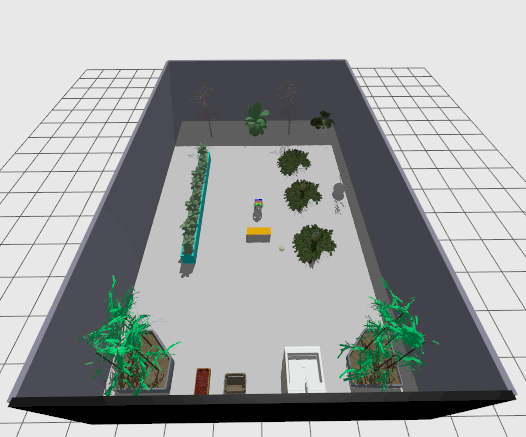
\includegraphics[width=1\textwidth]{figures/cap_4/mundo_invernadero.png}
  \caption{Mundo Invernadero para la aplicación}
  \label{fig:mundo_invernadero}
\end{figure}

Para llevar a cabo esta aplicación, simplemente se ha ido llamando a las funciones necesarias de la librería CoordMovesLib hasta conseguir el resultado esperado.

A continuación, en el \autoref{lst:aplicación} se muestra el código de esta aplicación para demostrar el uso de funciones de la librería y se adjunta un vídeo\footnote{\url{https://drive.google.com/file/d/149xjkhnO3WAhAMmqFwPOr-CfqX21xO_G/view?usp=sharing}} demostrativo de la misma, además de un par de  fotos para que se parecie mejor en la \autoref{fig:aplicacion_1} y también en la \autoref{fig:aplicacion_2}.

\begin{lstlisting}[language=Python, caption={Aplicación GreenNao}, label={lst:aplicación}, numbers=left, backgroundcolor=\color{gray!10}]
import CoordMovesLib
import time

time.sleep(5)
CoordMovesLib.grab_box()
time.sleep(3)

for i in range(3):
  CoordMovesLib.turn("L", 60)

CoordMovesLib.turn("L", 40)

CoordMovesLib.setArc(1, 0)
time.sleep(3)

CoordMovesLib.release_box()
print("Terminado")
\end{lstlisting}

\begin{figure}[H]
  \centering
  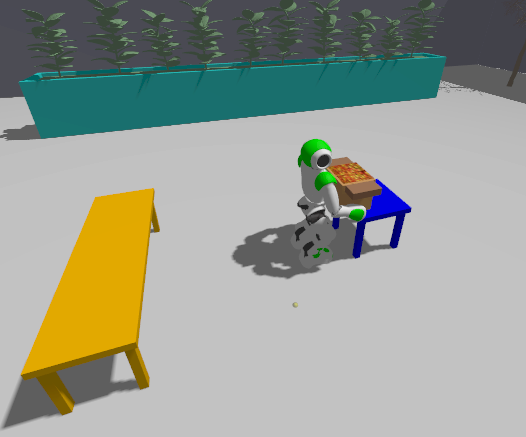
\includegraphics[width=0.7\textwidth]{figures/cap_4/app_1.png}
  \caption{Aplicación GreenNao. Vista lateral}
  \label{fig:aplicacion_1}
\end{figure}

\begin{figure}[H]
  \centering
  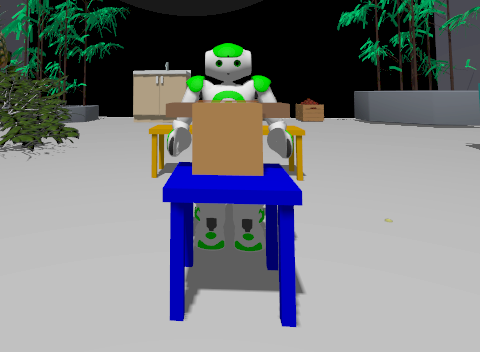
\includegraphics[width=0.7\textwidth]{figures/cap_4/app_2.png}
  \caption{Aplicación GreenNao. Vista frontal}
  \label{fig:aplicacion_2}
\end{figure}
    \chapter{Conclusiones}\label{cap:conclusiones}

Una vez visto lo que se ha hecho en este proyecto, se procede a concluir si se han cumplido o no los objetivos, y que posibilidades de mejora tiene para el futuro. Sin olvidar las competencias adquiridas y utilizadas para su desarrollo.

\section{Cumplimiento del objetivo}

Ya visto el desarrollo completo del proyecto, podemos decir que efectivamente se ha cumplido el objetivo final, debido a que se han cumplido cada uno de los subobjetivos.

Se ha alcanzado el subobjetivo 1, mencionado en el Capítulo \ref{cap:objetivos}, ya que se desarrolló un editor basado en secuencias de fotogramas (explicado en el Capítulo \ref{cap:capa_movimiento}). Este editor permite organizar referencias de posición para cada uno de los actuadores que participan en el movimiento coordinado, en la locomoción basado KME, como se describe en el Capítulo \ref{subsec:editor}.

Además, se ha desarrollado un intérprete capaz de comunicarse con los controladores individuales de cada articulación para que las replique, como bien se ha visto en el Capítulo \ref{subsec:interprete}. El resultado de esto es que se puede ver que el robot es capaz de saludar, levantarse, coger la caja, etc.

El subobjetivo 2, también explicado en el  Capítulo \ref{cap:objetivos}, se ha visto cumplido en el Capítulo \ref{cap:capa_movimiento}, mediante las clases de la librería que permiten la entrada de parámetros y modifican los tiempos de ejecución de los movimientos. Esto se ve claramente en las secuencias de caminata recta de 10 pasos, de caminata lateral, la caminata en arco, las funciones de coger y dejar la caja, los saludos, las formas de levantarse, etc. Estas secuencias dotan al robot de una primera capa de locomoción que permite programar sus movimientos(ya sean fijos o parametrizables) en aplicaciones robóticas de modo razonablemente simple, sin que el desarrollador tenga que programar explícitamente la coordinación de todos los actuadores individuales involucrados.Todo esto gracias a la librería desarrollada para ello.

Y, por último, también se ha cumplido el subobjetivo 3, también explicado en el Capítulo \ref{cap:objetivos}, porque, como se ha visto en el Capítulo \ref{sec:aplicacion}, ha quedado resuelta, demostrándonos que NAO cumple con los requisitos requeridos: La manipulación de la caja a la hora de recogerla y dejarla en su lugar de destino y el hecho de ser capaz de caminar con ella en brazos.

\section{Competencias empleadas}

Estos objetivos se han cumplido gracias a los conocimientos adquiridos a la hora de cursar las siguientes asignaturas de mi grado:

\begin{itemize}
    \item \textit{Modelado y Simulación de robots}: En esta asignatura se trata cómo funciona una simulación robótica, en términos generales, utilizando ROS2 y Gazebo.
    \item \textit{Arquitecturas Software para robots}: Asignatura dedicada a enseñarnos a utilizar ROS2 y programar con este middleware.

    \item \textit{Laboratorio de sistemas}: En esta asignatura aprendimos a manejar el sistema operativo Ubuntu,  utilizado en este TFG. Además de enseñarnos a utilizar la herramnienta \textit{git} para el manejo de repositorios remotos de Github.

    \item \textit{Robótica de servicios}: En esta asignatura nos enseñaron los fundamentos de los robots de servicio y su forma de programarlos.

    \item \textit{Fundamentos de la programación}: En esta asignatura aprendimos a manejar el lenguaje Python. 
    
\end{itemize}

\section{Competencias adquiridas}

Este proyecto ha hecho que adquiera diferentes competencias, útiles para diferentes campos de la robótica en general.

La primera de ellas ha sido la capacidad de encapsular ROS2 mediante una librería, cosa que es útil para desarrollar capas de control de cualquier tipo para cualquier sistema que utilice este middleware. Este conocimiento no entra en ninguna asignatura vista en el grado.

La segunda ha sido la capacidad de desarrollar un mundo completo para Gazebo, ya que, aunque como se mencionó en la sección anterior que se utilizaron los conocimientos aduiridos en la asignatura \textit{Modelado y simuación de robots}, el diseño del mundo no entraba en el itinerario de la asignatura. Así como el uso íntegro de Gazebo Harmonic (los puentes con ROS2, los plugins necesarios para adaptar el modelo, etc), debido a que en esta asignatura se trabajó con una versión anterior.

También se ha adquirido la capacidad de tratar con ficheros de formato JSON, ya que no había tratado con ellos anteriormente.

\section{Trabajos futuros}

Como trabajos futuros, tenemos un abanico bastante amplio de posibilidades.

En primer lugar, llevar este proyecto a un robot real. Cabe destacar que el trabajo en simulación también es válido y potente, sin embargo, no deja de ser algo que no existe del todo en la realidad, por lo que sería muy interesante hacer el paso conocido cómo \textit{sim 2 real}, para que un NAO real disponga de las funcionalidades que la librería de locomoción desarrollada ofrece.

Un segundo trabajo futuro, es hacer los modos de caminar más robustos y estables, ya que, como se ha visto en el Capítulo~\ref{cap:capa_movimiento}, hay algunos movimientos que no están del todo conseguidos (como es el caso de los arcos hacia atrás) o son algo inestables (como los demás modos de caminar). También se podría investigar para reducir el número de pasos mínimo. También sería interesante introducir funciones para la lectura de la cámara, como se mencionó en la sección \ref{subsec:sensores}

Un tercer posible trabajo futuro sería construir más aplicaciones de robótica de servicios con el robot NAO, creando más escenarios y desafíos para el robot. Esto sería interesante en el ámbito educativo, por ejemplo, para proponer prácticas a los estudiantes y que deban resolverlas utilizando la librería, siendo este abanico de posibilidades casi infinito.


    % Bibliografía
    \bibliographystyle{unsrtnat}
    \bibliography{bibliografia.bib}
        

% Fin del documento
\end{document}
